\section{基于 Bost--Charles 积分的更精细 holonomy 边界}\label{sec:8}

本节将第 6 节中的测度集中输入与第 7 节中的 Bost--Charles 精细化相结合, 给出了我们论文中所推导出的所有定理中最精确的广义 holonomy 边界. 
虽然对于定理 A 和 C 的特定应用, 额外增加的强度结果为零, 并且该定理的陈述变得有些复杂, 
但我们仍然希望抽象精细化的原理在未来的 holonomy 边界应用中会是有用的.

在第 2 节的框架下, 将高维方法引入 Bost--Charles 微积分中所带来的理论改进, 
正如我们所能告诉的那样, 仅仅体现在分母项 \(\tau(\mathbf{b}; \mathbf{e})\) 中. 
人们不可避免地会问, 第 6 节与第 7 节中的增长积分哪一个更小. 
在第 8.1 节中, 我们给出了由 Fedor Nazarov 提供的一个证明, 
该证明表明 Bost--Charles 积分严格优于重排积分. 
特别是, 根据我们启发性的注记 7.6.7, 这意味着定理 7.6.4 比定理 6.0.2 更为精确, 
至少就后者定理中所陈述的分母而言是这样的. 
（注记 6.6.15 指出, 第 6 节中的多维证明在一般分母方面可以比第 7 节走得更远, 并且至少与我们本节第 8 节的选择相一致.） 
本节下文的注记 8.1.17 表明, 阿基米德增长项之间的差异通常非常小, 
这意味着使用重排积分几乎不会损失任何精度. 
出于使用不同的映射 \(\varphi\) 对 holonomy 边界进行抽样和测试的目的, 
后一种积分在实际中具有允许进行更快且更可靠的数值计算的优势.

我们现在着手阐明我们的统一定理. 
\setcounter{footnote}{31}
以下总结了我们在本文中证明的所有 holonomy 边界中最尖锐的边界\footnote{可能取决于考虑除 \(\varphi_r\) 之外的其他 \(\varphi\), 如同在定理 6.0.2 或定理 7.1.13 中那样. 
此类变体同样可以直接纳入其中, 但我们在此不予展开.}.

\begin{theorem}\label{thm:8.0.1}
我们放宽定理 6.0.2 中关于分母的所有假设, 并且允许任意具有非负系数的分母矩阵 \(\mathbf{b} \in M_{m\times r}(\mathbf{R}^{\ge 0})\). 
定义
\begin{equation}\label{eq:8.0.2}
\tau^{\flat}(\mathbf{b}) := \limsup_{\epsilon \to 0, \varepsilon \to 0} \limsup_{d \to \infty} \left\{ \frac{1}{d} \limsup_{N \to \infty} \mathrm{Den}_{N}(\mathbf{b}, \epsilon, d, \varepsilon) \right\},
\end{equation}
\[ \mathrm{Den}_{N}(\mathbf{b}, \epsilon, d, \varepsilon) := \frac{2}{N} \sum_{k \in \mathbf{N}_{>0}} \max_{\mathbf{n} \in P_{\varepsilon}^{d}(N), \mathbf{i} \in V_{m}^{d}(\epsilon)} \#\{(j, h) : k \leq b_{i_{j}, h} \cdot n_{j}\}, \]
其中 \((j, h)\) 遍历 \(\{1, . . . , d\} \times \{1, . . . , r\}\), 
子集 \(V_m^d(\epsilon) \subset \{1, . . . , m\}^d\) 定义为:
\[
\begin{aligned}
V_m^d(\epsilon) := \big\{ &\mathbf{i} \in \{1, \dots, m\}^d : \forall i_0 \in \{1, \dots, m\}, \\
& d/m - \epsilon d < \#\{1 \le j \le d \mid i_j = i_0\} < d/m + \epsilon d \big\},
\end{aligned}
\]
并且 \(P_{\varepsilon}^{d}(N) \subset [0, N]^{d} \cap \mathbf{Z}^{d}\) 表示那些使得 \(\{n_{i}/N\}_{i=1}^{d}\) 的归一化 \(([0, 1), \mu_{\text{Lebesgue}})\) 偏差 \(\leq \varepsilon\) 的 \(\mathbf{n}\) 的子集.

假设要么
\[ \log |\varphi'(0)| > \max \left\{ \sum_{h=1}^r \max_{1 \leq i \leq m} b_{i,h}, \tau^{\flat}(\mathbf{b}) + \tau^{\sharp}(\mathbf{e}) \right\}, \]
要么 \(\log |\varphi'(0)| > \tau^{\flat}(\mathbf{b}) + \tau^{\sharp}(\mathbf{e})\) 且所有的 \(f_i\) 都是 holonomic.

那么我们有:
\begin{equation}\label{eq:8.0.3}
m \le \frac{\iint_{\mathbf{T}^2} \log |\varphi(z) - \varphi(w)| \, \mu_{\mathrm{Haar}}(z) \mu_{\mathrm{Haar}}(w)}{\log |\varphi'(0)| - (\tau^{\flat}(\mathbf{b}) + \tau^{\sharp}(\mathbf{e}))}.
\end{equation}
进一步, 对于定理 7.1.6 中的任意子半径序列 \(1 = r_l > r_{l-1} > \cdots > r_0 > 0\), 
且采用定义 7.1.2 的 Bost--Charles 特征 \(\widehat{T}\), 我们有:
\begin{equation}\label{eq:8.0.4}
m \leq \frac{\iint_{\mathbf{T}^2} \log |\varphi(z) - \varphi(w)| \, \mu_{\mathrm{Haar}}(z) \mu_{\mathrm{Haar}}(w) - \frac{1}{m} \sum_{k=1}^l \frac{(\widehat{T}(r_k, \varphi) - \widehat{T}(r_{k-1}, \varphi))^2}{\log r_k - \log r_{k-1}}}{\log |\varphi'(0)| - (\tau^{\flat}(\mathbf{b}) + \tau^{\sharp}(\mathbf{e}))}.
\end{equation}
此外, 如果对于给定的 \(\{r_k\}\), \(s_h^*\) 如同在定理 7.6.4 中那样定义, 那么我们有:
\begin{equation}\label{eq:8.0.5}
m \leq \frac{\iint_{\mathbf{T}^2} \log |\varphi(z) - \varphi(w)| \, \mu_{\mathrm{Haar}}(z) \mu_{\mathrm{Haar}}(w) - \sum_{h=0}^{l-1} s_h^* \cdot (\widehat{T}(1, \varphi) - \widehat{T}(r_h, \varphi))}{\log |\varphi'(0)| - (\tau^{\flat}(\mathbf{b}) + \tau^{\sharp}(\mathbf{e}))}.
\end{equation}
\end{theorem}

\begin{remark}\label{rem:8.0.6}
我们根据定义观察到 \(\tau^{\flat}(\mathbf{b}) \in [0, \infty)\). 
更确切地, 我们有自明边界 \(\tau^{\flat}(\mathbf{b}) \leq \sum_{h=1}^{r} \max_{i=1}^{m} \{b_{i,h}\}\).

对于在第 6--7 节中通篇考虑的形式的分母矩阵 \(\mathbf{b}\), 我们有 \(\tau^{\flat\flat}(\mathbf{b}) = \tau^{\flat}(\mathbf{b})\). 
事实上, 记 t 为离散变量 \(k/N\) 的连续极限, 
我们在定理 6.0.2 的设定中拥有 \(\tau^{\flat\flat}(\mathbf{b})\) 被下式所上控制:
\[ \sum_{h=1}^{r} \limsup_{\epsilon, \varepsilon \to 0} \limsup_{d \to \infty} \left\{ \frac{1}{d} \limsup_{N \to \infty} \left\{ \frac{2}{N} \sum_{k \in \mathbb{N}_{>0}} \max_{\mathbf{n} \in P_{\varepsilon}^{d}(N), \mathbf{i} \in V_{m}^{d}(\epsilon)} \#\{(j, h) : k \leq b_{i_{j}, h} \cdot n_{j}\} \right\} \right\} \]
\[ \leq 2 \sum_{h=1}^{r} \int_{0}^{b_{h}} \min\{1 - u_{h}/m, 1 - t/b_{h}\} dt = \sum_{h=1}^{r} \left(b_{h} - \frac{b_{h}u_{h}^{2}}{m^{2}}\right) = \tau^{\flat}(\mathbf{b}), \]
其中不等式源于以下观察：对均衡的 \(\mathbf{i}\) （意味着：每个 \(i_0 \in \{1, \ldots, m\}\) 渐近出现的频率为 1/m）的限制在第二行的被积函数中提供了上界约束 \(1 - u_h/m\), 
而对均衡的 \(\mathbf{n}\) （意味着：分量集合 \(\{n_j\}\) 渐近地取 \([0, N]\) 上的均匀分布）的限制在该被积函数中提供了上界约束 \(1 - t/b_h\). 
此外, 当 \(\mathbf{n}\) 和 \(\mathbf{i}\) 都按非降序排列时（即 \(n_1 \leq \cdots \leq n_d\) 且 \(i_1 \leq \cdots \leq i_d\)）, 不等式取到等号. 
这证明了在第 6 节和第 7 节通篇所作的常规假设下, 有 \(\tau^{\flat\flat}(\mathbf{b}) = \tau^{\flat}(\mathbf{b})\). 
（另请参见引理 6.6.7 和注记 6.6.14.） \end{remark}

\begin{example}\label{ex:8.0.7}
这里有一个简单的例子来说明，对于给定的 \(\mathbf{b}\), 
如果让 \(\mathbf{b}'\) 遍历所有在系数上支配 \(\mathbf{b}' \geq \mathbf{b}\) 且另外满足定理 6.0.2 约束的数组, 
不等式 \(\tau^{\flat\flat}(\mathbf{b}) \leq \tau^{\flat}(\mathbf{b}')\) 可以是严格的.

考虑 \(\mathbf{b} = [0, 1, 2]^{\mathrm{t}}\). 为了使用 \(\tau^{\flat}\), 
\(\mathbf{b}'\) 的最优选择是取 \(\mathbf{b}' = [0, 2, 2]^{\mathrm{t}}\) 且我们有 \(\tau^{\flat}(\mathbf{b}') = \frac{16}{9}\). 
另一方面, 我们有 \(\tau^{\flat\flat}(\mathbf{b}) = \frac{5}{3} = \frac{15}{9}\).

事实上, 记 \(t := k/N\), 我们有:
\[ \tau^{\flat\flat}(\mathbf{b}) = 2\left(\int_0^{2/3} \frac{2}{3} dt + \int_{2/3}^1 \left(1 - t + \frac{1}{3}\right) dt + \int_1^{4/3} \frac{1}{3} dt + \int_{4/3}^2 \left(1 - \frac{t}{2}\right) dt\right). \]
这需要与下式进行比较:
\[ \tau^{\flat}(\mathbf{b}') = 2 \int_0^2 \min\left\{\frac{2}{3}, 1 - \frac{t}{2}\right\} dt. \]
为了解释两个公式之间的差异, 我们注意到在范围 \(t \in [2/3, 4/3]\) 内, 
对于在 \(\tau^{\flat\flat}(\mathbf{b})\) 的定义中要考虑的每一个 \(\mathbf{n}\), 
在 \(n_j\) 中至多有 \((\max\{0, 1-t\} + o(1))d\) 个带有 \(i_j = 2\) （对应于 \(b_{2,1} = 1\)）的项对 \(\{(j,1) \mid k \leq n\}\) 产生贡献, 
且在 \(n_j\) 中至多有 \((1/3 + o(1))d\) 个带有 \(i_j = 3\) （对应于 \(b_{3,1} = 2\)）的项对 \(\{(j,1) \mid k \leq 2n\}\) 产生贡献, 
并且通过对 \(\mathbf{n}\) 的合适选择, 两个边界都可以达到. \end{example}

\subsection{Bost--Charles 积分与重排积分的比较}\label{sec:8.1}

本节内容完全由 Fedor Nazarov 贡献, 旨在对两种积分进行干净的比较——这是基于我们在附录 A 中遇到的情况以及在大多数多价情况下实践中观察到的它们实际上是相同的经验性观察. 
严格来说, 本定理对于我们在本文中的任何证明都没有被使用, 
因此它在第一次阅读（以及第二次阅读）中是可以被略去的.

\begin{remark}[Basic Remark 8.1.1]\label{rem:8.1.1}
由于接下来的考虑依赖于平面上的位势理论, 我们首先考虑在最简易的 Lie 群——圆周 \(\mathbf{T}\)——上的更容易情况. 
可积函数 \(G(z) := \log \frac{1}{|1-z|}\), \(G: \mathbf{T} \to \mathbf{R} \cup \{\infty\}\) 拥有非负 Fourier 系数:
\begin{equation}\label{eq:8.1.2}
\widehat{G}(n) := \int_{\mathbf{T}} G(z) z^{-n} \, \mu_{\text{Haar}}(z) = \int_{\mathbf{T}} z^{-n} \log \frac{1}{|1 - z|} \, \mu_{\text{Haar}}(z) = \begin{cases} 0, & \text{如果 } n = 0; \\ \frac{1}{2|n|}, & \text{如果 } n \neq 0. \end{cases}
\end{equation}
根据一般的 Bochner 定理, Fourier 变换的正性意味着 \(G(z)\) 在局部紧 abelian 群 \(\mathbf{T}\) 上是一个正定函数： 
即对于所有在 \(\mathbf{T}\) 上的合理的带符号测度 \(\nu\), 均有 \(\iint_{\mathbf{T}^2} G(zw^{-1}) \nu(z) \nu(w) \geq 0\). 
这里的合理可以被理解为 \(\nu = \nu^+ - \nu^-\) 且满足 \(\int_{\mathbf{T}} G \nu^\pm < \infty\) 的有限正测度 \(\nu^\pm\). 
对于任何此类带符号测度 \(\nu\), 这一计算更确切地表明:
\begin{equation}\label{eq:8.1.3}
\begin{aligned}
I(\nu) &:= \iint_{\mathbf{T}^2} \log \frac{1}{|z - w|} \nu(z) \nu(w) \\
&= \iint_{\mathbf{T}^2} \log \frac{1}{|1 - zw^{-1}|} \nu(z) \nu(w) \\
&= \sum_{n \in \mathbf{Z} \setminus \{0\}} \frac{|\widehat{\nu}(n)|^2}{2|n|} \ge 0,
\end{aligned}
\end{equation}
显然, 等号成立当且仅当 Fourier 变换 \(\widehat{\nu}\) 是在 \(\widehat{\mathbf{T}} = \mathbf{Z}\) 的零元素 \(0\) 处的 Dirac 质量的标量倍数, 
并且反过来, 这发生当且仅当 \(\nu\) 是 Haar 测度 \(\mu_{\text{Haar}}\) 的标量倍数. 
这反映了圆周上的基本位势理论. \end{remark}

在任意半径 \(R\) 的圆周 \(|z| = R\) 上, \eqref{eq:8.1.3} 的左手边在相差一个加项 \((\log R) (\int \nu)^2\) 的意义下进行缩放, 
因此对于 \(R > 1\), 虽然对于该圆周支撑的任意测度 \(\nu\) 不等式 \eqref{eq:8.1.3} 是错误的, 
但它对于满足 \(\int \nu = \nu(\mathbf{C}) = 0\) 的那些均衡（balanced）测度仍然是成立的. 
由于对数核在加法平移下也是不变的, 后一评述对于在 \(\mathbf{C}\) 中的任何圆周携带的均衡测度也仍然是成立的.

正如我们接下来要回顾的, 能量积分的正性是关于 \(\mathbb{C}\) 上均衡测度的一个完全普遍的事实.

\subsubsection{能量原理}\label{sec:8.1.4}

在由 \(\mathbf{0} \in \mathbf{R}^n\) 处的点质量创建的 Newtonian 引力场中, 位能函数 \(U : \mathbf{R}^n \setminus \{\mathbf{0}\} \to \mathbf{R}\) 
由分布拉普拉斯方程决定:
\[ \Delta U := \sum_{i=1}^{n} \frac{\partial^2 U}{\partial x_i^2} = -\delta_0, \]
即作为该方程的基本解 \(U := U_n^2\), 其中更一般地, 考虑由下式定义的 \emph{Riesz 位势} \cite{Rie38} 是有用的:
\begin{equation}\label{eq:8.1.5}
U_n^{\alpha}(\mathbf{x}) := \begin{cases} \frac{\Gamma\left(\frac{n}{2}\right)}{2\pi^{\frac{n}{2}}} \log \frac{1}{\|\mathbf{x}\|}, & \text{对于 } n = \alpha; \\ \frac{\Gamma\left(\frac{n-\alpha}{2}\right)}{2^{\alpha}\Gamma\left(\frac{\alpha}{2}\right)\pi^{\frac{n}{2}}} \frac{1}{\|\mathbf{x}\|^{n-\alpha}}, & \text{对于 } n > \alpha > 0. \end{cases}
\end{equation}
此处, \(\|\mathbf{x}\| := \sqrt{\sum_{i=1}^n x_i^2}\) 是 \(\mathbf{R}^n\) 中的欧几里得距离函数. 
引力位势 \(U = U_n^2\) 是旋转不变的, 并且定义了一个核函数 \(k(\mathbf{x},\mathbf{y}) := U_n^2(\mathbf{x}-\mathbf{y})\), 
根据定义, 它此外也是平移不变的. 
对于 \(n>2\), 该核也是正定的, 这源于 Frostman 和 Marcel Riesz 的基本公式 \cite[第 I.3 节]{Rie38}, 
该公式推广了 Dirichlet 能量积分 \(\frac{1}{2} \iiint \|\nabla F\|^2\) dvol, 
并等价于对 \(U_n^2\) 的分布 Fourier 变换的计算 \cite{Den50}\cite{Sch66}\cite{Lan72}\cite{NS91}:
\begin{equation}\label{eq:8.1.6}
I(\nu) := \iint_{\mathbf{R}^n \times \mathbf{R}^n} k(\mathbf{x}, \mathbf{y}) \, \nu(\mathbf{x}) \nu(\mathbf{y}) = \iint_{\mathbf{R}^n \times \mathbf{R}^n} U_n^2(\mathbf{x} - \mathbf{y}) \, \nu(\mathbf{x}) \nu(\mathbf{y}) = \int_{\mathbf{R}^n} \left( U_n^1 * \nu \right)^2 \, \mu_{\text{Lebesgue}}.
\end{equation}
这是圆周上能量公式 \eqref{eq:8.1.3} 的空间模拟. 
更确切地, 这一公式给出了在 \(\mathbf{R}^n\) 上任意非零紧支撑带符号测度 \(\nu = \nu^+ - \nu^-\) 
（可表示为具有收敛能量积分 \(I(\nu^+), I(\nu^-) < \infty\) 的两个有限正 Borel 测度 \(\nu^+, \nu^-\) 的差） 
的能量严格正性 \(I(\nu) > 0\). 
对于对数核（\(n=2\) 的情况, 其在物理上的正确解释实际上是板上的静电学）, 
Riesz 观察到 \cite[第 I.4 节]{Rie38}, 在额外要求带符号测度 \(\nu\) 均衡（即 \(\nu(\mathbf{R}^2) = 0\)）的前提下, 
与圆周的类比变得几乎完美. 
能量原理指出, 对于在满足上述正则性条件的均衡带符号测度（在 \(n=2\) 的情况下, 均衡条件是唯一必需的）, 
能量 \(I(\nu) \geq 0\) 是非负的, 并且等号成立当且仅当 \(\nu=0\). 
这精细化了紧集平衡概率测度的唯一性定理. \(n=2\) 的情况（这也是我们所关心的）在 \cite[定理 16.4.2]{Hil62} 中有详细讨论.

\subsubsection{Fuglede 不等式}\label{sec:8.1.7}

为了完备起见, 我们总结了由 Fuglede \cite{Fug60} 给出的关于非均衡测度的更一般情况. 
这是关于 \(n=2\) 的情况向 \(\mathbb{R}^n\) 上的对数核
\[ k(\mathbf{x}, \mathbf{y}) := U_n^n(\mathbf{x} - \mathbf{y}) = \frac{\Gamma(n/2)}{2\pi^{n/2}} \log \frac{1}{\|\mathbf{x} - \mathbf{y}\|} \]
的另一种推广. 对于这一对数核, 对应于均衡测度情况的能量公式的模拟也是由 Riesz 给出的 \cite[第 I.4 节]{Rie38}:
\[ \int_{\mathbf{R}^n} \nu = 0 \quad \Longrightarrow \quad I(\nu) = \int_{\mathbf{R}^n} \left( U_n^{n/2} * \nu \right)^2 \, \mu_{\text{Lebesgue}} \ge 0, \]
并且更一般地, Fuglede \cite[第 4 节]{Fug60} 证明了尖锐的能量下界:
\begin{equation}\label{eq:8.1.8}
I(\nu) \ge \log\left(\frac{a_n}{R}\right) \cdot \left(\int_{\mathbf{R}^n} \nu\right)^2,
\end{equation}
这对于在 \(\mathbf{R}^n\) 上所有可表示为 \(\nu = \nu^+ - \nu^-\) （伴随着具有收敛能量积分 \(I(\nu^\pm) < \infty\) 的有限正测度 \(\nu^\pm\), 
且具有支撑集 \(\operatorname{supp}(\nu) \subseteq \{\|\mathbf{x}\| \leq R\}\)）的带符号测度 \(\nu\) 都是有效的, 
其中最优常数 \(a_n\) 恰好为:
\[ a_n := \begin{cases} \exp\left(\frac{1}{2} + \dots + \frac{1}{n-4} + \frac{1}{n-2}\right), & \text{对于 } n \text{ 偶数;} \\ \exp\left(\frac{1}{1} + \dots + \frac{1}{n-4} + \frac{1}{n-2} - \log 2\right), & \text{对于 } n \text{ 奇数.} \end{cases} \]
\(a_1 = 1/2\) 以及 \(a_2 = 0\) （对于我们所关心的 \(n = 2\) 的情况）的情况已经在 de la Vall{\'e}e-Poussin 的工作中给出 \cite[第 47 节]{dlVP49}. 
在任何情况下, \eqref{eq:8.1.8} 显然意味着对于所有（合理的）均衡测度, 并且更一般地, 
对于由足够小的球支撑的所有测度, 所必需的正性 \(I(\nu) \geq 0\) 都是成立的.

\subsubsection{Michelli 关于正定核的准则}\label{sec:8.1.9}

另一种推广（我们参考 \cite{Mat97} 以及那里的参考文献）允许任意具有 \(k(\mathbf{x}, \mathbf{y}) = U(\|\mathbf{x} - \mathbf{y}\|)\) 形式的核, 
其中 \(U(t) \in C^{\infty}(\mathbf{R}_{>0})\) 对于所有 \(n \geq n_0\) 服从 \((-1)^n \left(\frac{d}{dt}\right)^n U(t) \geq 0\), 
且现在在 \(\mathbf{R}^d\) 上紧支撑的带符号测度 \(\nu = \nu^+ - \nu^-\) （伴随着 \(I(\nu^{\pm}) < \infty\)）上的额外（``均衡''）约束为： 
对于所有满足 \(|\mathbf{m}| < n_0\) 的 \(\mathbf{m} \in \mathbf{N}^d\), 均有 \(\int_{\mathbf{R}^d} \mathbf{x}^{\mathbf{m}} \nu(\mathbf{x}) = 0\). 
关于 \(U(t)\) 的条件等价于存在一个关于在 \(\mathbf{R}_{>0}\) 上的正 Borel 测度 \(d\alpha\) 的 Laplace--Stieltjes 变换的 \(\left(\frac{d}{dt}\right)^{n_0} U(t) = \int_0^{\infty} e^{-tu} d\alpha(t)\) 积分表示.

\subsubsection{相交配对与标号}\label{sec:8.1.10}

非正式地总结这一讨论\footnote{如果我们要将更一般的核 k(x,y) 纳入其中, 那么这在第 8.1.9 节中是取 \(n_0 := 1\). 
对于算术几何, 相关的案例是 n = 2 且核 \(k(z, w) = -\log|z - w|\).}的另一种方式是说, 
在 \(\mathbb{R}^n\) 上的合理（非均衡）带符号测度空间上, 
无限维二次型
\[ \langle \mu, \nu \rangle := \iint_{\mathbf{R}^n \times \mathbf{R}^n} k(\mathbf{x}, \mathbf{y}) \, \mu (\mathbf{x}) \nu(\mathbf{y}) \]
恰好具有一个 `\(-\)' 号. 
对于我们关心的 \(n=2\) 的情况（这也是 8.1 节其余部分相关的案例）, 
如果能与 Arakelov 理论中的算术 Hodge 指标公式以及在 \cite[第 5 节]{BC22} 中导出 Bost--Charles 双重积分的计算建立起更精确的联系, 
那将会是非常有趣的. 
是否存在一个直接在 \cite{BC22} 算术相交理论框架内起作用的 Nazarov 不等式（下面的命题 8.1.13）的证明？ 
在代数模型中的一个基本评述是：对于在一个极化的正规射影代数曲面上的任意两个线丛 L 和 M, 
如果 \((L.L) = (M.M)\) 且 \(\deg L = \deg M\), 
那么根据针对线丛 \(L \otimes M^{-1}\) 的 Hodge 指标定理, 有 \((L.L) \leq (L.M)\).

\subsubsection{Nazarov 不等式}\label{sec:8.1.11}

现在考虑将 \(n=2\) 的情况作为复平面 \(\mathbf{R}^2 \cong \mathbf{C}\). 
那么旋转群是通过由圆周点 \(a\in \mathbf{T}\) 索引的幺正变换 \(t_a: z\mapsto az\) 实现的, 
并且我们的旋转不变、正定核在 \(\mathbf{C}\) 上具有我们所描述的正则性条件的均衡带符号测度线性空间上由 \(k(z,w)=\frac{1}{2\pi}\log\frac{1}{|z-w|}\) 给出. 
我们考虑一个非常数连续函数 \(\varphi:\mathbf{T}\to\mathbf{C}\), 
并且对于任何 \(a\in \mathbf{T}\), 我们应用能量原理 \(I(\nu)\geq 0\) 于均衡带符号测度 \(\nu=\nu_a:=\varphi_*(\mu_{\mathrm{Haar}})-t_a^*\varphi_*(\mu_{\mathrm{Haar}})\). 
由于核 \(k(z,w)\) 是对称且旋转不变的, 由此产生的不等式重新改写为:
\begin{equation}\label{eq:8.1.12}
\begin{aligned}
&\iint_{\mathbf{T}^2} \log |\varphi(z) - \varphi(w)| \, \mu_{\text{Haar}}(z) \mu_{\text{Haar}}(w) \\
&\quad \le \iint_{\mathbf{T}^2} \log |a\varphi(z) - \varphi(w)| \, \mu_{\text{Haar}}(z) \mu_{\text{Haar}}(w),
\end{aligned}
\end{equation}
对于任何 \(a \in \mathbf{T}\) 均成立, 并且等号成立当且仅当 \(\nu_a = 0\). 对 \(a \in \mathbf{T}\) 积分我们得到:

\begin{proposition}[Nazarov]\label{prop:8.1.13}
对于任意连续函数 \(\varphi : \mathbf{T} \to \mathbf{C}\),
\[
\begin{aligned}
&\iint_{\mathbf{T}^2} \log |\varphi(z) - \varphi(w)| \, \mu_{\text{Haar}}(z) \mu_{\text{Haar}}(w) \\
&\quad \leq \iint_{\mathbf{T}^2} \log \max \left( |\varphi(z)|, |\varphi(w)| \right) \, \mu_{\text{Haar}}(z) \mu_{\text{Haar}}(w) \\
&\quad = \int_0^1 2t \cdot (\log |\varphi(e^{2\pi i t})|)^* \, dt,
\end{aligned}
\]
其中 \(g^*\) 表示一个连续函数 \((0,1) \to \mathbf{R}\) 的递增重排 \eqref{eq:2.4.1}. 
此外, 等号成立当且仅当 \(\varphi(z) = cz^m\) 对于某个 \(c \in \mathbf{C}\) 以及 \(m \in \mathbf{Z}\).
\end{proposition}

\begin{proof}
在 \eqref{eq:8.1.12} 的项向积分 \(\int_{\mathbf{T}} I(\nu_a) \, \mu_{\text{Haar}}(a) \geq 0\) 中使用 Poisson 公式
\[ \int_{\mathbf{T}} \log|ax - y| \,\mu_{\text{Haar}}(a) = \log \max(|x|, |y|). \]
等号成立要求对于几乎所有的 \(a \in \mathbf{T}\) 均有 \(\nu_a = 0\), 
从而 \(\varphi_*(\mu_{\text{Haar}})\) 是旋转不变的, 
并因此支撑回路 \(\varphi(\mathbf{T}) \subset \mathbf{C}\) 是一个以原点为中心的圆周, 
并且 \(\varphi^*(\mu_{\text{Haar}})\) 是该圆周上 Haar 测度的标量倍数.
\end{proof}

特别是, 我们得到了一个干净的证明, 
表明 Bost--Charles 积分总是被我们在 \cite{CDT24} 中所拥有的、加倍的 Nevanlinna 特征严格控制（而不单单是被 \cite[命题 5.4.5]{BC22} 中所指出的、稍微大一些的加倍的 Ahlfors--Shimizu 特征
\[ \int_{\mathbf{T}} \log \sqrt{1 + |\varphi|^2} \, \mu_{\text{Haar}} \]
所控制, 后者是一个更基本的估计, 仅仅遵循平凡的逐点不等式 \(|x - y|^2 \le (1 + |x|^2)(1 + |y|^2)\)）:

\begin{corollary}\label{cor:8.1.14}
每个连续函数 \(\varphi : \mathbf{T} \to \mathbf{C}\) 都满足
\[ \iint_{\mathbf{T}^2} \log |\varphi(z) - \varphi(w)| \, \mu_{\mathrm{Haar}}(z) \mu_{\mathrm{Haar}}(w) \leq 2 \int_{\mathbf{T}} \log^+ |\varphi| \, \mu_{\mathrm{Haar}}. \]
\end{corollary}

\begin{figure}[htbp]
  \centering
  \centering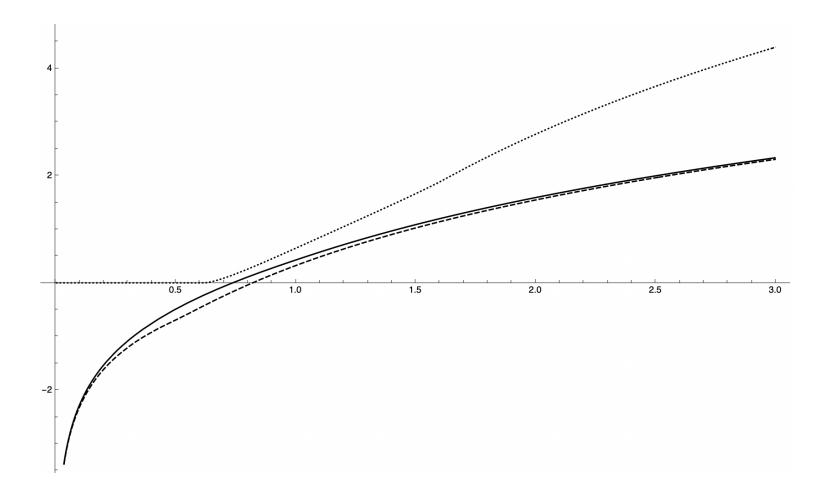
\includegraphics[width=0.8\textwidth]{assets/fig/_page_127_Figure_2.jpeg}
  \caption{针对二价函数 \(\varphi_r(z) = (rz) - (rz)^2\), 重排积分（实线）与 Bost--Charles 积分（虚线）的函数图像. 在它们上方（点线）为 \(2 \int_{\mathbf{T}} \log^+ |\varphi_r| \, \mu_{\text{Haar}}\) 的函数图像.}\label{fig:8.1.15}
\end{figure}

\begin{example}\label{ex:8.1.16}
考虑具有变化半径 r 的函数 \(\varphi_r(z) := rz - (rz)^2\). 
对于 \(r \ge 1\), Bost--Charles 积分等价于:
\[ \iint_{\mathbf{T}^2} \log |\varphi_r(z) - \varphi_r(w)| \, \mu_{\text{Haar}}(z) \mu_{\text{Haar}}(w) = 2 \log r + \int_{\mathbf{T}} \log^+ \left| \frac{r}{1 - rz} \right| \mu_{\text{Haar}}(z) \]
\[ = 2 \log r + \frac{1}{\pi r} + \frac{1}{72\pi r^2} + \dots \]
相比之下, 对重排积分的计算揭示其作为显式函数为:
\[ \int_{0}^{1} 2t \cdot (\log |\varphi_{r}(e^{2\pi it})|)^{*} dt = 2\log r + \frac{1}{2\pi^{2}} \left(8\operatorname{Li}_{3}(1/r) - \operatorname{Li}_{3}(1/r^{2})\right) \]
\[ = 2\log r + \frac{4}{\pi^{2}r} + \frac{4}{27\pi^{2}r^{2}} + \dots \]
这一比较对于 r 的大多数值而言都是非常紧密的, 如\autoref{fig:8.1.15} 所示. 
相比之下, 通过下式给出的 Nevanlinna 特征上界:
\[ 2\int_{\mathbf{T}} \log^+ |\varphi_r| \, \mu_{\text{Haar}} = 2\int_{|z|=r} \log^+ |z - z^2| \, \mu_{\text{Haar}}(z) \]
\[ = 4\log r \quad \text{当 } r \ge \frac{\sqrt{5} + 1}{2} \text{ 时} \]
是非常粗糙的. \end{example}

\begin{remark}\label{rem:8.1.17}
两种增长特征积分在“大”半径 \(|z| = r\) 处的渐近等价性（如在示例 8.1.16 和\autoref{fig:8.1.15} 中所观察到的）似乎是一个相当普遍的特征, 
它反映了膨胀圆周 \(|z| = r\) 的均匀测度 \(\mu_{\text{Haar}}\) 在 \(\varphi_*\) 下推前测度的近乎旋转不变性, 
这考虑到通过切片不等式 \eqref{eq:8.1.12} 对命题 8.1.13 的证明. 
一个“在实际中”的例子见于我们在第 14.5 节中对定理 C 的证明. 
在在这种情况下, Bost--Charles 积分 \eqref{eq:A.6.1} 与重排积分 \eqref{eq:A.6.3} 的比较如下:
\[ 9.963 \sim \iint_{\mathbf{T}^2} \log |\varphi(z) - \varphi(w)| \, \mu_{\text{Haar}}(z, w) \leq \int_0^1 2t \cdot (\log |\varphi(e^{2\pi i t})|)^* \, dt \, \sim 9.972, \]
这是一个仅在千分之几数量级上的改进.
（相比之下, 来自 \eqref{eq:B.0.2} 的 Nevanlinna 特征量 \(2T(\varphi) = 2 \int_{\mathbf{T}} \log^+ |\varphi| \mu_{\mathrm{Haar}}\) 在当前情况下大到 \(\sim 14.08\).）

这一类的另一个例子可以通过比较源于定理 6.0.2 以及定理 7.6.4 的、在定理 A 的两个证明中出现的上界来观察到. 
通过定理 6.0.2 的证明（带有两个划分点, 参见第 13 节）给出了关于重排积分形式的边界 \(m < 13.731\). 
在另一方面, 定理 7.6.4 给出了关于算术相交数形式的边界, 
这些相交数可表示为作为 Bost--Charles 积分轻微推广的积分（参见引理 7.4.5）. 
伴随着对划分点类似的选取, 这导致了边界 \(m < 13.679\) （参见示例 7.6.8, 特别是公式 \eqref{eq:7.6.9}）, 
这是一个小于百分之零点五的改进. 
由于凸性论证引起的积分和边界的轻微修改形式, 这一比较字面上并不是命题 8.1.13 的例子. 
然而, 它准确地反映了我们在没有凸性下数值上观察到的、在重排积分和 Bost--Charles 积分之间的改进程度. \end{remark}

\subsection{定理 8.0.1 的证明}\label{sec:8.2}

我们首先证明 \eqref{eq:8.0.4}, 它将 \eqref{eq:8.0.3} 作为一个特殊情况包含在内. 
我们将在最后讨论如何修改证明以获得 \eqref{eq:8.0.5}.

对于下文, 我们固定一个 \(\epsilon > 0\) 以及变量个数 d. 
仅仅在证明的最后, 我们将首先令 \(d \to \infty\), 随后令 \(\epsilon \to 0\). 
为了与第 6 节和 \eqref{eq:6.0.10} 进行比较, 
我们指出定理 8.0.1 中的边界在使用高维等分布特征的前提下, 在分母中仅具有 \(\tau^{\flat\flat}(\mathbf{b})\), 
而其他项与第 7 节中推导出的单变量边界是相同的. 
因此, 为了证明定理 8.0.1, 我们只需要纳入在 \(\prod_{j=1}^d f_{i_j}(x_j)\) 中均衡指标 \(\mathbf{i} = (i_1, \dots, i_d)\) 的特征, 
而我们不需要像第 6.2 节中那样在 \(\mathbf{x}^{\mathbf{k}}\) 中使用等分布的次数 k. 
这启发了我们要作为我们的评估模基础的欧几里得格的以下选择.

\subsubsection{欧几里得格}\label{sec:8.2.1}

考虑自由 \(\mathbf{Z}\)-模:
\begin{equation}\label{eq:8.2.2}
E_D := \bigoplus_{\mathbf{i} \in V_m^d(\epsilon)} f_{\mathbf{i}}(\mathbf{x}) \mathbf{Z}[1/x_1, \dots, 1/x_d]_{\leq D},
\end{equation}
其中我们召回, 子集 \(V_m^d(\epsilon) \subset \{1, \dots, m\}^d\) （取决于固定的微小正整常数 \(\epsilon\)）定义为
\[
\begin{aligned}
V_m^d(\epsilon) = \Big\{ \mathbf{i} \in \{1, \dots, m\}^d &: \forall i_0 \in \{1, \dots, m\}, \\
& d/m - \epsilon d < \#\{1 \le j \le d \mid i_j = i_0\} < d/m + \epsilon d \Big\};
\end{aligned}
\]
并且按惯例, \(f_{\mathbf{i}}(\mathbf{x}) := \prod_{j=1}^d f_{i_j}(x_j)\). 
在此, \(\mathbf{Z}[1/x_1, \dots, 1/x_d]_{\leq D}\) 表示由 \(1/x_1, \dots, 1/x_d\) 组成的整多项式组成的自由 \(\mathbf{Z}\)-模, 
其中所有的偏次数——对于每个 \(1/x_j\)——都至多为 D.

根据构造, 有 \(\operatorname{rank} E_D = (D+1)^d \cdot \#V_m^d(\epsilon)\). 
根据定理 4.2.1（实际上, 大数弱定律在此处已足够）, 我们有:
\[ \lim_{d\to\infty} \frac{\#V_m^d(\epsilon)}{m^d} = 1, \quad \text{因此} \quad \lim_{d\to\infty} \lim_{D\to\infty} \frac{\operatorname{rank} E_D}{m^d D^d} = 1. \]

为了赋予 \(E_D\) 适当的范数, 我们考虑光滑射影算术方案 \(\mathcal{X} := (\mathbf{P}_{\mathbf{Z}}^1)^d\) 
以及在 \(\mathcal{X}\) 上的自然极宽裕线丛 \(\mathcal{L} := \otimes_{j=1}^d \operatorname{pr}_j^* \mathcal{O}(1)\), 
其中 \(\operatorname{pr}_j : \mathcal{X} \to \mathbf{P}_{\mathbf{Z}}^1\) 表示投影到第 j 个分量上的态射. 
那么我们可以将 \(\Gamma(\mathcal{X}, \mathcal{L}^{\otimes D})\) 识别为 \(\mathbf{Z}[1/x_1, \ldots, 1/x_d]_{\leq D}\), 
其中 \(x_j := Y_j/Z_j\) 是第 j 个 \(\mathbf{P}_{\mathbf{Z}}^1 = \operatorname{Proj} \mathbf{Z}[Y_j, Z_j]\) 的仿射坐标.

召回我们被给予了一个全纯映射 \(\varphi: (\overline{\mathbf{D}}, 0) \to (\mathbf{P}^1(\mathbf{C}), 0)\), 
其中 ``0'' 可以意味着对于每个在 \(\mathcal{X}_{\mathbf{C}}\) 中的 \(\mathbf{P}^1_{\mathbf{C}}\) 副本均有 \(x_j = 0\). 
来自第 7.3.1 节的 Bost--Charles 度量因此通过在每个因子 \(\operatorname{pr}^*_j \, \mathcal{O}(1)\) 上使用 \(\varphi\) 来定义. 
这在 \(\mathcal{L}\) 上诱导了一个 Hermitian 线丛结构 \(\overline{\mathcal{L}} = (\mathcal{L}, \|\cdot\|_{\overline{\mathcal{L}}})\), 
并且反过来, 如同在第 7.3.3 节中一样, 在我们固定了 \((\mathbf{P}^1)^d(\mathbf{C})\) 上的光滑概率测度 \(\nu\) 之后, 
在 \(\mathbf{Z}\)-模 \(\Gamma(\mathcal{X}, \mathcal{L}^{\otimes D})\) 上定义了一个欧几里得格 \(\Gamma_{L^2}\left(\mathcal{X}, \nu; \overline{\mathcal{L}}^{\otimes D}\right)\). 
\(\nu\) 的选择对于证明是无足轻重的, 
因为我们只需在固定的 \(\nu\) 下令 \(D \to \infty\), 
并且我们只需要研究由对于 \(\widehat{\deg} \Gamma_{L^2}\left(\mathcal{X}, \nu; \overline{\mathcal{L}}^{\otimes D}\right)\) 
的算术 Hilbert--Samuel 公式给出的渐近领先阶数项. 
具体而言, 我们选取 \(\nu\) 为光滑测度:
\[
\begin{aligned}
\nu &:= \bigwedge_{j=1}^{d} \operatorname{pr}_{j}^{*} \omega_{\mathrm{FS}} \\
&= \left(\frac{\sqrt{-1}}{2\pi}\right)^{d} \frac{dz_{1} \wedge \cdots \wedge dz_{d} \wedge d\bar{z}_{1} \wedge \cdots \wedge d\bar{z}_{d}}{\prod_{j=1}^{d} (1+|z_{j}|^{2})^{2}},
\end{aligned}
\]
伴随着 \(\omega_{\text{FS}} = \frac{\sqrt{-1}}{2\pi} \frac{dz \wedge d\bar{z}}{(1+|z|^2)^2}\) 为在 \(\mathbf{P}^1(\mathbf{C})\) 上的 Fubini--Study 形式. 
那么, 如第 7.3.3 节所示, 在 \(\Gamma\left(\mathcal{X},\overline{\mathcal{L}}^{\otimes D}\right)\) 上的欧几里得范数 \(\|\cdot\|\) 由下式定义:
\begin{equation}\label{eq:8.2.3}
||s|| := \sqrt{\int_{\mathcal{X}(\mathbf{C})} ||s||_{\mathcal{L}}^2 \nu}.
\end{equation}

正如在第 7.3.3 节中一样, 我们取以下由 \eqref{eq:8.2.3} 在 \(\Gamma\left(\mathcal{X}, \overline{\mathcal{L}}^{\otimes D}\right)\) 上的诱导范数所给出的欧几里得格的正交直和 \eqref{eq:8.2.2}:
\[
\begin{aligned}
&\mathbf{Z}[1/x_1,\ldots,1/x_d]_{\leq D} \\
&\quad \cong \Gamma(\mathcal{X},\mathcal{L}^{\otimes D}) \subset \Gamma(\mathcal{X},\mathcal{L}^{\otimes D})_{\mathbf{R}}.
\end{aligned}
\]
我们将这一欧几里得格记为 \(\overline{E}_D = (E_D, \|\cdot\|)\).

\subsubsection{算术度}\label{sec:8.2.4}

直接像到 Spec \(\mathbf{Z}\) 的算术度的渐近计算是算术 Hilbert--Samuel 公式的研究主题:

\begin{lemma}\label{lem:8.2.5}
当 \(D \to \infty\) 时, 我们有关于算术度如下的渐近性:
\begin{equation}\label{eq:8.2.6}
\widehat{\operatorname{deg}} \, \Gamma_{L^{2}} \left( \mathcal{X}, \nu; \overline{\mathcal{L}}^{\otimes D} \right) = \frac{d}{2} \left( \overline{\mathcal{O}(1)} \cdot \overline{\mathcal{O}(1)} \right) D^{d+1} + o(D^{d+1}),
\end{equation}
\[ \widehat{\operatorname{deg}} \, \overline{E}_{D} = \frac{d \# V_{m}^{d}(\epsilon)}{2} \left( \overline{\mathcal{O}(1)} \cdot \overline{\mathcal{O}(1)} \right) D^{d+1} + o(D^{d+1}). \]
\end{lemma}

\begin{proof}
作为欧几里得格, \(\Gamma(\mathcal{X}, \overline{\mathcal{L}}^{\otimes D}) \cong \bigotimes_{j=1}^{d} \Gamma\left(\mathbf{P}_{\mathbf{Z}}^{1}, \overline{\mathcal{O}(1)}^{\otimes D}\right)\), 
其中每一因子 \(\Gamma\left(\mathbf{P}_{\mathbf{Z}}^{1}, \overline{\mathcal{O}(1)}^{\otimes D}\right)\) 上的范数都是使用 Hermitian 线丛 \(\overline{\mathcal{O}(1)}\) 
以及在 \(\mathbf{P}^1(\mathbf{C})\) 上的 Fubini--Study 形式 \(\omega_{\text{FS}}\) 的 \(L^2\)-范数. 
因此, 根据引理 7.2.7, 我们有
\[ \widehat{\operatorname{deg}}\,\Gamma\left(\mathcal{X},\overline{\mathcal{L}}^{\otimes D}\right) = d(D+1)^{d-1}\widehat{\operatorname{deg}}\,\Gamma\left(\mathbf{P}_{\mathbf{Z}}^{1},\overline{\mathcal{O}(1)}^{\otimes D}\right). \]
现在, 第一个断言源于算术 Hilbert--Samuel 公式 \eqref{eq:7.3.4}. 
第二个断言根据 \eqref{eq:7.2.4} 源于第一个断言.
\end{proof}

\begin{remark}\label{rem:8.2.7}
这一计算的证明也是 Krull 维度为 d+1 的一般算术 Hilbert--Samuel 公式的推论. 
在 \cite[定理 1.4]{Zha95} 中, 算术 Hilbert--Samuel 公式对于任意维度的算术簇以及配备有逐点非负 Chern 形式的光滑度量的宽裕 Hermitian 线丛得到了证明. 
利用 \cite[第 5 节]{Bos99} 和 \cite[第 3--4 节]{BC22} 中的想法, 
相同的公式对于在任意维度的算术簇上、配备有逐点非负 Chern 形式的 \(\mathcal{C}^{\mathrm{b}\Delta}\) Hermitian 度量的宽裕线丛仍然是成立的. 
因此我们也可以直接从关于 \((\mathcal{X}, \overline{\mathcal{L}})\) 的算术 Hilbert--Samuel 公式推导引理 8.2.5:
\[ \widehat{\operatorname{deg}}\,\Gamma_{L^2}\left(\mathcal{X},\nu;\overline{\mathcal{L}}^{\otimes D}\right) = \frac{\overline{\mathcal{L}}^{d+1}}{(d+1)!}D^{d+1} + o(D^{d+1}). \]
在此, \(\overline{\mathcal{L}}^{d+1}\) 表示算术自相交数 \(\widehat{c}_1(\overline{\mathcal{L}})^{d+1}.[\mathcal{X}]\). 
在我们的设定中, 我们写出 \(\overline{\mathcal{L}} = \otimes_{j=1}^d \operatorname{pr}_j^* \overline{\mathcal{O}(1)}\), 
并通过多线性展开自相交数. 唯一非零项来自于对除了一个 \(\operatorname{pr}_{i}^{*}\mathcal{O}(1)\) 因子之外的所有因子穿过一次, 
以及对剩下的这一个 \(\operatorname{pr}_{i}^{*}\mathcal{O}(1)\) 因子穿过两次. 
根据投影公式, 这为我们提供了
\[ \overline{\mathcal{L}}^{d+1} = d \binom{d+1}{2} (d-1)! \left( \overline{\mathcal{O}(1)} \cdot \overline{\mathcal{O}(1)} \right), \]
并且我们以此透视同样恢复了引理 8.2.5. \end{remark}

\subsubsection{评估过滤}\label{sec:8.2.8}

记 \(X := \mathcal{X}_{\mathbf{Q}}\), 我们可以将 \(\operatorname{Spf} \mathbf{Q}[\![x]\!] = \widehat{X}_0\) 识别为 X 在其闭子模式 0 处的形式完备化, 
这特别地对于 \(i = 1, \dots, m\) 给出了元素
\[ f_{\mathbf{i}} = f_{\mathbf{i}}(\mathbf{x}) \in \Gamma(\widehat{X}_0, \mathcal{O}_{\widehat{X}_0}). \]
\(\mathcal{L}^{\otimes D}|_{\widehat{X}_0}\) 的全局截面空间 \(\Gamma\left(\widehat{X}_0, \mathcal{L}^{\otimes D}\right)\) 随后被自然地识别为:
\[
\begin{aligned}
\Gamma\left(\widehat{X}_0, \mathcal{L}^{\otimes D}\right) &= \mathbf{x}^{-D}\mathbf{Q}[\![\mathbf{x}]\!] \\
&=: F_{\mathbf{Q}},
\end{aligned}
\]
其中 \(\mathbf{x}^{-D}\mathbf{Q}[\![\mathbf{x}]\!]\) 表示由满足对于所有 \(1 \leq j \leq d\) 均有 \(k_j \geq -D\) 
的 \(\mathbf{x}^{\mathbf{k}}\) 组成的 \(\mathbf{Q}\)-向量空间. 
因此 \(f_{\mathbf{i}} \Gamma(\mathcal{X}, \mathcal{L}^{\otimes D}) \subset \Gamma(\widehat{X}_0, \mathcal{L}^{\otimes D})\), 
并且我们有单射评估映射:
\[ \psi_D: E_D \hookrightarrow F_{\mathbf{Q}}, \quad (Q_{\mathbf{i}})_{\mathbf{i} \in V_m^d(\epsilon)} \mapsto \sum_{\mathbf{i} \in V_m^d(\epsilon)} f_{\mathbf{i}} Q_{\mathbf{i}}, \]
此处的 \(Q_{\mathbf{i}} \in \Gamma(\mathcal{X}, \mathcal{L}^{\otimes D})\) 且 \((Q_{\mathbf{i}})_{\mathbf{i} \in V_m^d(\epsilon)} \in E_D\). 
与第 3.1.3 节类似, 我们首先使用总消逝阶数、随后在每个射流空间（jet space）内使用字典序来过滤 \(F_{\mathbf{Q}}\):
\[ F_{\mathbf{Q}} = F_{\mathbf{Q}}^{(\mathbf{0})} \supseteq \cdots \supseteq F_{\mathbf{Q}}^{(\mathbf{n})} \supseteq \cdots, \]
其中 \(\mathbf{n} \in \mathbf{N}^d\), 并且 \(F_{\mathbf{Q}}^{(\mathbf{n})} := \operatorname{Span}_{\mathbf{Q}}\{\mathbf{x}^{\mathbf{m}} : \mathbf{n} \prec \mathbf{m} + D \text{ 或 } \mathbf{n} = \mathbf{m} + D\}\). 
在此处, \(\mathbf{N}^d\) 上的总序 \(\prec\) 定义在第 3.1.3 节中, 并且对于 \(\mathbf{m} = (m_j)_{j=1}^d\), 
我们定义 \(\mathbf{m} + D := (m_j + D)_{j=1}^d\). 
用于定义字典序的变量 \(x_1, \ldots, x_d\) 的顺序对于证明是无足轻重的. 
在这一 \(\prec\)-过滤记号下, 由于 \(\prod_{j=1}^d x_j^{-D} \in \Gamma(\mathcal{X}, \mathcal{L}^{\otimes D})\) 
是 \(\mathcal{L}_0^{\otimes D}\) 的一个生成元（此处我们用 \(\mathcal{L}_0\) 表示 \(\mathcal{L}\) 到 \(\mathbf{Z}\)-点 \(\mathbf{x} = \mathbf{0}\) 的限制）, 
我们观察到：一个形式截面 \(g(\mathbf{x}) \in F_{\mathbf{Q}} = \Gamma(\widehat{X}_0, \mathcal{L}^{\otimes D})\) 
在 \(\mathbf{x} = \mathbf{0}\) 处的消逝阶数 \(\operatorname{ord}_0(g(\mathbf{x}))\) （作为 \(\mathcal{L}^{\otimes D}|_{\widehat{X}_0}\) 的正则截面, 
而不是作为 \(\mathbf{x}^{-D}\mathbf{Q}[\![\mathbf{x}]\!]\) 中的 Laurent 级数） 
至少为 n, 当且仅当 \(g(\mathbf{x}) \in F_{\mathbf{Q}}^{(0,\ldots,0,n)}\). 
我们还观察到 \(g(\mathbf{x}) \in F_{\mathbf{Q}}^{(\mathbf{n})}\) 当且仅当要么 \(\operatorname{ord}_0(g(\mathbf{x})) > |\mathbf{n}|\), 
要么 \(\operatorname{ord}_0(g(\mathbf{x})) = |\mathbf{n}|\) 并且在 g 的齐次度为 \(|\mathbf{n}|\) 的部分中最低字典序项具有指数向量 \(\mathbf{m}\), 
使得 \(\mathbf{n} \prec \mathbf{m}\). 
（如果在此处人们更倾向于将 g 视为 \(\mathbf{x}^{-D}\mathbf{Q}[\![\mathbf{x}]\!]\) 中的 Laurent 级数, 
而不是作为 \(\mathcal{L}^{\otimes D}|_{\widehat{X}_0}\) 的形式截面, 
那么在这些陈述中, 人们将不得不把所有的指数向量 \(\mathbf{n}\) 平移到 \(\mathbf{n} - D\).）

与第 3.1.3 节类似, 我们用 \(\mathbf{n}^+\) 表示 \(\mathbf{n}\) 在总序 \(\prec\) 下的后继. 
Graded 分量 \(F_{\mathbf{Q}}^{(\mathbf{n})}/F_{\mathbf{Q}}^{(\mathbf{n}^+)}\) 是一个一维 \(\mathbf{Q}\)-向量空间, 
由商映射下 \(\mathbf{x}^{\mathbf{n}-D}\) 的像所生成. 
在 \(F_{\mathbf{Q}}^{(\mathbf{n})}/F_{\mathbf{Q}}^{(\mathbf{n}^+)}\) 上的欧几里得格结构由商映射下 \(\mathbf{x}^{\mathbf{n}-D}\) 
的像所生成的自由秩 1 \(\mathbf{Z}\)-模以及满足 \(\|\mathbf{x}^{\mathbf{n}-D}\| = 1\) 的欧几里得范数所给出. 
除了在 x 的幂次中有一个 \(-D\) 的移动之外, 这与第 7.3 节中是相同的.

正如在第 7.3 节中一样, 我们拥有自然的单射评估映射 \(\psi_D: E_D \to F_{\mathbf{Q}}\), 
这在 graded 分量上诱导了单射:
\[ \psi_D^{(\mathbf{n})}: E_D^{(\mathbf{n})}/E_D^{(\mathbf{n}^+)} \hookrightarrow F_{\mathbf{Q}}^{(\mathbf{n})}/F_{\mathbf{Q}}^{(\mathbf{n}^+)}. \]
因此对于所有 \(\mathbf{n} \in \mathbf{N}^d\), 
均有 \(\operatorname{rank} E_D^{(\mathbf{n})}/E_D^{(\mathbf{n}^+)} \in \{0,1\}\). 
令
\[ \mathcal{V}_D^d := \{ \mathbf{n} \in \mathbf{N}^d \mid \operatorname{rank} E_D^{(\mathbf{n})} / E_D^{(\mathbf{n}^+)} = 1 \} \]
为消逝过滤跳跃集合. 我们有 \(\#\mathcal{V}_D^d = \operatorname{rank} E_D\).

在接下来的第 8.2.11 节和第 8.2.29 节中, 我们提供关于在所有 \(v \in M_{\mathbf{Q}}\) 处的局部评估高度 \(h_v(\psi_D^{(\mathbf{n})})\) 的上界估计. 
根据局部评估高度的定义, 我们需要考虑任意的 \((Q_{\mathbf{i}})_{\mathbf{i} \in V_m^d(\epsilon)} \in E_D^{(\mathbf{n})} \setminus E_D^{(\mathbf{n}^+)}\), 
并随后提供 \(\log |c_{\mathbf{n}}|_v - \log ||(Q_{\mathbf{i}})_{\mathbf{i} \in V_m^d(\epsilon)}||_{E_D,v}\) 的上界, 
其中 \(c_{\mathbf{n}}\) 表示在 \(s := \sum_{\mathbf{i} \in V_m^d(\epsilon)} f_{\mathbf{i}}Q_{\mathbf{i}}\) 中 \(\mathbf{x}^{\mathbf{n}-D}\) 的系数. 
在此处, \(|c_{\mathbf{n}}|_v\) 表示在 \(\mathbf{Q}\) 上的常用 v-进范数.

\begin{definition}\label{def:8.2.9}
对于域 k 上的形式幂级数 \(F(t_1, \ldots, t_d) \in k[\![t_1, \ldots, t_d]\!] = \sum_{\mathbf{n}} a_{\mathbf{n}} \mathbf{t}^{\mathbf{n}}\), 
F 的 n-阶射流（jet）是由所有次数为 n 的项之和给出的、次数为 n 的齐次多项式 \(J_n(F) \in k[t_1, \ldots, t_d]_{(n)}\):
\[ J_n(F)(t_1,\ldots,t_d) := \sum_{| \mathbf{n} | = n} a_{\mathbf{n}} \mathbf{t}^{\mathbf{n}} \in k[\mathbf{t}]_{(n)}. \]
\end{definition}

\begin{remark}\label{rem:8.2.10}
在关于高维形式解析算术簇代数化的早期工作 \cite{Bos01}\cite{Bos04} 中, 
仅使用在点 \(\mathbf{0}\) 处的总消逝阶数来过滤辅助评估模就已经足够了. 
我们在此使用具有一维商的更精细过滤, 该做法具有两个优势:
\begin{itemize}
  \item[(1)] 对于在阿基米德地方 v 处 \(h_v\) 的估计, 
  利用 \(\overline{\mathbf{D}}^d \to \mathcal{X}(\mathbf{C})\) 的乘积结构, 
  我们拥有与 \cite[引理 2.4.1]{CDT21} 类似的一个容易的“逐个变量”次调和估计. 
  这避免了 \cite[第 4.3.2 节]{Bos01} 中的吹起方法, 
  后者给出了领先阶数射流多项式 \(J_n(F) \in \mathbf{Q}[\mathbf{x}]_{(n)}\) 的 Mahler 测度的上界, 
  而需要被估计的量是该领先阶数射流中单个系数 \(c_{\mathbf{n}}\) 的大小. 
  在维度 \(d = \dim \mathcal{X}_{\mathbf{Q}}\) 中, 这些量的差异是非常敏感的, 
  维度 d 在 \cite{Bos01} 中是固定的, 
  而在我们的方法中, 我们希望最后令 \(d \to \infty\).
  \item[(2)] 在非阿基米德地方 v 处对 \(h_v\) 估计的优势是至关重要的. 
  在满足 \(|\mathbf{n}| = n\) 的所有 \(\mathbf{n}\) 中, 
  由于我们对 \(E_D\) 的特定构造, 我们在 \(\{n_j\}_{j=1}^d\) 渐近等分布分量的条件下将拥有对 \(h_v\left(\psi_D^{(\mathbf{n})}\right)\) 的好得多的估计. 
  我们包含字典序的完全过滤允许我们利用这一改进. \end{itemize}
\end{remark}

\subsubsection{阿基米德估计}\label{sec:8.2.11}

召回通过与引理 7.4.1 证明开端的相同简化论证, 
我们对于所有 \(1 \le i \le m\), 都可以假设 \(f_i(\varphi(z))\) 
在 \(|z| \le 1\) 的一个开邻域上是亚纯的.

为了方便记号, 我们用 \(|\cdot|\) 表示常用绝对值 \(|\cdot|_{\infty}\). 
证明的更宽框架与 \cite[第 4.3.3 节]{Bos01} 类似, 
并带有着我们在注记 8.2.10(1) 中描述的修改. 
给定 \(s \in \psi_D^{(\mathbf{n})}(E_D^{\mathbf{n}} \setminus E_D^{\mathbf{n}^+})\), 
我们将遵循 \cite[第 2.4 节]{CDT21} 中关于研究在点 \(\mathbf{z} = \mathbf{0} \in \overline{\mathbf{D}}^d\) 
处的 \(n\)-阶（领先）射流 \(J_n(\varphi^*s)(\mathbf{z}) \in \mathbf{C}[\mathbf{z}]_{(n)}\). 
在此处以及在下文中, 我们使用记号 \(n := |\mathbf{n}|\), 
并且伴随着对记号的轻微滥用, 我们继续用 \(\varphi : \overline{\mathbf{D}}^d \to \mathcal{X}(\mathbf{C})\) 
表示在每个因子上对角定义的解析态射 \(\mathbf{x} \mapsto (\varphi(z_1), \dots, \varphi(z_d))\) （此处 \(\varphi : \overline{\mathbf{D}} \to \mathbf{C}\)）. 
通过该记号的推广, 并且以统一第 6 节和第 7.4 节的方式, 
我们对于每个 \(\mathbf{r} \in (0, 1]^d\) 考虑解析态射:
\[ \varphi_{\mathbf{r}}: \overline{\mathbf{D}}^d \to \mathbf{C}^d \hookrightarrow \mathcal{X}(\mathbf{C}), \qquad \mathbf{z} \mapsto (\varphi(r_1 z_1), \dots, \varphi(r_d z_d)). \]
我们将使用 Poisson--Jensen 公式通过射流函数来约束 \(\log |c_{\mathbf{n}}|\), 
随后借助 Poincaré--Lelong 公式将产生的边界与 \(\overline{\mathcal{L}}\) 的 Chern 形式联系起来. 
我们遵循第 7.4 节中的记号, 并且我们从 \eqref{eq:7.1.7} 借用斜率 \(\alpha_k\) 的记号. 
此外, 对于每个 \(\mathbf{n} \in \mathbf{N}^d\), 我们定义 \(r(\mathbf{n}) := (r(n_1), \ldots, r(n_d))\), 
其中
\begin{equation}\label{eq:8.2.12}
r(t) := \begin{cases} r_k, & t/D \in [\alpha_k, \alpha_{k+1}), \\ 1, & t/D > m. \end{cases}
\end{equation}

通篇本节, \(\mathbf{z} = (z_1, \dots, z_d)\) 表示 \(\overline{\mathbf{D}}^d\) 上的坐标. 
我们使用通过 \(\mathbf{x}^{-D} \mapsto \mathbf{1}\) 给出的、\(\mathcal{L}^{\otimes D}\) 在 \(\mathbf{A}^d_{\mathbf{C}}\) 
上的平凡化 \(\mathcal{L}^{\otimes D}|_{\mathbf{C}^d} \stackrel{\simeq}{\to} \mathcal{O}_{\mathbf{C}^d}\). 
在此识别下, \(s/\mathbf{x}^{-D} = s \cdot \mathbf{x}^D =: G(\mathbf{x})\) 
自然在 \(\Gamma(\widehat{X}_0, \mathcal{O}_{\widehat{X}_0})\) 中且消逝阶数为 n. 
由于我们解析的 \(\varphi_{r(\mathbf{n})}\)-拉回是由 \(x_j = \varphi_{r(n_j)}(z_j) = (\varphi'(0) \cdot r(n_j))z_j + O(z_j^2)\) 定义的, 
我们根据构造有 \(\varphi^*_{r(\mathbf{n})}G\) 具有 \(\mathbf{z} = \mathbf{0}\) 消逝阶数 n, 
并且在 \(J_n\left(\varphi_{r(\mathbf{n})}^*G\right)\) 
中（以及在 \(\varphi_{r(\mathbf{n})}^*G\) 中的整体 \(\prec\)-极小项） 
以 \(c_{\mathbf{n}}\varphi'(0)^n \prod_{j=1}^d r(n_j) \mathbf{z}^{\mathbf{n}}\) 
为字典序极小项. 
然而, 由于我们在此定理中仅假设了拉回函数的*亚纯性*（而不是全纯性）： \(\varphi^*f_i \in \mathcal{M}(\overline{\mathbf{D}})\), 
解析芽 \(\varphi_{r(\mathbf{n})}^*G \in \mathbf{C}[\![\mathbf{z}]\!]\) 
仅亚纯地（而不是全纯地）延拓通过 \(\overline{\mathbf{D}}\). 
但如果我们选择全纯函数 \(h \in \mathcal{O}(\overline{\mathbf{D}})\), 
满足 \(h(0) = 1\) 且所有的 \(h \cdot \varphi^*f_i \in \mathcal{O}(\overline{\mathbf{D}})\) 都是全纯的, 
那么 \(h(z_1) \cdots h(z_d) \cdot \left(\varphi_{r(\mathbf{n})}^*\right) G(\mathbf{z}) \in \mathcal{O}\left(\overline{\mathbf{D}}^d\right)\) 
在整个 \(\overline{\mathbf{D}}^d\) 上是全纯的, 
并且具有与 \(\varphi_{r(\mathbf{n})}^*G\) 相同的领先阶数射流 \(J_n\left(\varphi_{r(\mathbf{n})}^*G\right)\).

这使我们可以利用 \cite[引理 2.4.1]{CDT21} 来根据齐次多项式 \(J_n\left(\varphi_{r(\mathbf{n})}^*G\right) = J_n\left(h(z_1)\cdots h(z_d)\cdot \varphi_{r(\mathbf{n})}^*G\right)\) 
的 Mahler 测度来上估计所必需的系数 \(|c_{\mathbf{n}}|\), 
在其中显然整体上字典序最低的项是在多重次数 \(\mathbf{n}\) 中的单项式 \(c_{\mathbf{n}}\mathbf{z}^{\mathbf{n}}\):
\begin{equation}\label{eq:8.2.13}
\begin{aligned}
\log |c_{\mathbf{n}}| &\leq -n \log |\varphi'(0)| - \sum_{j=1}^{d} n_{j} \log r(n_{j}) \\
&\quad + \int_{\mathbf{T}^{d}} \log \left| J_{n} \left( h(z_{1}) \cdots h(z_{d}) \cdot \varphi_{r(\mathbf{n})}^{*} G \right) \right| \mu_{\text{Haar}}.
\end{aligned}
\end{equation}

我们可以将此与 Bost 在 \cite[引理 4.13 中的等式 (4.28)]{Bos01} 中的吹起论证联系起来, 该论证显示:
\begin{equation}\label{eq:8.2.14}
\begin{aligned}
&\int_{\mathbf{T}^d} \log \left| J_n \left( h(z_1) \cdots h(z_d) \cdot \varphi_{r(\mathbf{n})}^* G \right) \right| \mu_{\text{Haar}} \\
&\quad \leq \int_{\mathbf{T}^d} \log \left| h(z_1) \cdots h(z_d) \cdot \varphi_{r(\mathbf{n})}^* G \right| \mu_{\text{Haar}} \\
&\quad = \int_{\mathbf{T}^d} \log \left| \varphi_{r(\mathbf{n})}^* G \right| \mu_{\text{Haar}} + O_h(1).
\end{aligned}
\end{equation}
为了回顾 Bost 的论证, 写出 \(h(z_1) \cdots h(z_d) \cdot G(\varphi_{r(\mathbf{n})}^*(\mathbf{z})) =: \sum_{\mathbf{k} \in \mathbf{N}^d} c_{\mathbf{k}}' \mathbf{z}^{\mathbf{k}}\), 并定义:
\begin{equation}\label{eq:8.2.15}
U_t(\mathbf{z}) := \sum_{\mathbf{k} \in \mathbf{N}^d} c_{\mathbf{k}}' t^{|\mathbf{k}| - n} \mathbf{z}^{\mathbf{k}}, \quad \text{对于满足 } |t| \le 1 \text{ 的 } t \in \mathbf{C}.
\end{equation}
那么, 通过 \(\mathbf{z} \mapsto t\mathbf{z}\) 代换有:
\begin{equation}\label{eq:8.2.16}
\begin{aligned}
&\int_{\mathbf{T}^d} \log |U_t(\mathbf{z})| \, \mu_{\text{Haar}}(\mathbf{z}) \\
&= \int_{|t|\mathbf{T}^d} \log \left| h(z_1) \cdots h(z_d) \right. \\
&\quad \cdot \left. \varphi_{r(\mathbf{n})}^* G \right| \, \mu_{\text{Haar}}(\mathbf{z}) - n \log |t|.
\end{aligned}
\end{equation}
特别地, \(\int_{\mathbf{T}^d} \log |U_t(\mathbf{z})| \, \mu_{\text{Haar}}(\mathbf{z})\) 根据 \eqref{eq:8.2.15} 
显然是单复变量 t 的次调和函数, 
其仅通过等式 \eqref{eq:8.2.16} 右手边的等式依赖于该复变量 t （通过 \(|t|\)）. 
因此, 该函数在 t = 1 处的值（等于 \(\int_{\mathbf{T}^d} \log |h(z_1) \dots h(z_d) \cdot \varphi_{r(\mathbf{n})}^* G |\mu_{\text{Haar}}|\), 
但也是 \(\int_{\mathbf{T}^d} \log |U_t(\mathbf{z})| \, \mu_{\text{Haar}}(\mathbf{z})\) 在 \(t \in \mathbf{T}\) 上的积分） 
不小于其在 t = 0 处的值, 
后者正是所需边界 \eqref{eq:8.2.14} 的左手边.

接下来我们遵循 \cite[定理 10.5.3]{Bos20} 的证明想法, 
以及 \cite[第 4.2--4.3 节]{BC22} 中的讨论, 以便从光滑 Green 函数通过 \(\mathcal{C}^{b\Delta}\) 函数. 
通过 \(\overline{\mathcal{L}}\) 的乘积结构和引理 7.4.1 证明中的计算, 我们有:
\begin{equation}\label{eq:8.2.17}
\begin{aligned}
&\int_{\mathbf{T}^{d}} \log \|\varphi_{r(\mathbf{n})}^{*} \mathbf{x}^{-D}\|_{(\varphi_{r(\mathbf{n})}^{*}\overline{\mathcal{L}})} \mu_{\text{Haar}} \\
&= \sum_{j=1}^{d} \int_{\mathbf{T}} \log \|\varphi_{r(n_{j})}^{*}(x_{j}^{-D})\|_{\overline{\mathcal{O}(D)}} \mu_{\text{Haar}} \\
&= \sum_{j=1}^{d} \left( -\int_{\overline{\mathbf{D}}} \log^{+} |z|^{-1} c_{1} \left( \varphi_{r(n_{j})}^{*} \overline{\mathcal{O}(D)} \right) \right. \\
&\quad + \left. \|\varphi_{r(n_{j})}^{*}(x^{-D})\|_{\varphi_{r(n_{j})}^{*} \overline{\mathcal{O}(D)}} \Big|_{z=0} \right).
\end{aligned}
\end{equation}
由于 \(x^{-D}|_{x=0}\) 是自由 \(\mathbf{Z}\)-模 \(\mathcal{O}(D)_0\) 的一个 \(\mathbf{Z}\)-生成元, 我们有
\[ \|\varphi_{r(n_j)}^*(x^{-D})\|_{\overline{\mathcal{O}(D)}}\,\Big|_{z=0} = -\widehat{\operatorname{deg}}\,\overline{\mathcal{O}(D)}_0 = -D\,\widehat{\operatorname{deg}}\,\overline{\mathcal{O}(1)}_0. \]

结合 \eqref{eq:8.2.13}, \eqref{eq:8.2.14} 和 \eqref{eq:8.2.17}, 我们有:
\begin{equation}\label{eq:8.2.18}
\begin{aligned}
&\log |c_{\mathbf{n}}| - \int_{\mathbf{T}^{d}} \log \|\varphi_{r(\mathbf{n})}^{*}s\|_{(\varphi_{r(\mathbf{n})}^{*}\overline{\mathcal{L}})} \mu_{\mathrm{Haar}} \\
&\quad \leq -n \log |\varphi'(0)| - \sum_{j=1}^{d} n_{j} \log r(n_{j}) \\
&\qquad + \int_{\mathbf{T}^{d}} \left( \log |\varphi_{r(\mathbf{n})}^{*}G(\mathbf{z})| - \log \|\varphi_{r(\mathbf{n})}^{*}s\|_{\varphi_{r(\mathbf{n})}^{*}\overline{\mathcal{L}}} \right) \mu_{\mathrm{Haar}} + O_{h}(1) \\
&\quad = -n \log |\varphi'(0)| - \sum_{j=1}^{d} n_{j} \log r(n_{j}) - \int_{\mathbf{T}^{d}} \log \|\varphi_{r(\mathbf{n})}^{*}\mathbf{x}^{-D}\|_{(\varphi_{r(\mathbf{n})}^{*}\overline{\mathcal{L}})} \mu_{\mathrm{Haar}} + O_{h}(1) \\
&\quad = -n \log |\varphi'(0)| - \sum_{j=1}^{d} n_{j} \log r(n_{j}) \\
&\qquad + D \left( \sum_{j=1}^{d} \widehat{\deg}(\overline{\mathcal{O}(1)}_{0}) + \int_{\overline{\mathbf{D}}} \log^{+} |z|^{-1} c_{1}(\varphi_{r(n_{j})}^{*}\overline{\mathcal{O}(1)}) \right) + O_{h}(1)
\end{aligned}
\end{equation}
\[ = -n \log |\varphi'(0)| - \sum_{j=1}^{d} n_{j} \log r(n_{j}) + D \sum_{j=1}^{d} \widehat{T}(r(n_{j}), \varphi) + O_{h}(1), \]
其中 \(\widehat{T}(r(n_j), \varphi)\) 是我们定义在 \ref{def:7.1.2} 中的 Bost--Charles 特征, 
并且最后的等号源于对 \cite[命题 7.2.2]{BC22} 投影公式应用于注记 7.3.2 以及引理 7.4.5 中的态射 \((\iota, \varphi_{r(n_j)})\) 得到的. 
我们更详细地阐明最后一步. 
根据 \cite[第 7.1.1.1 节]{BC22} 中 Hermitian 向量丛拉回的定义以及 \cite[等式 6.2.4]{BC22} 中算术相交数的定义, 
我们有:
\[ (\iota, \varphi_{r(n_j)})^* \overline{\mathcal{O}(1)} \cdot ([0], \log^+|z|^{-1}) = \widehat{\operatorname{deg}} \, \overline{\mathcal{O}(1)}_0 + \int_{\overline{\mathbf{D}}} \log^+|z|^{-1} c_1(\varphi^*(\overline{\mathcal{O}(1)})). \]
通过 \cite[命题 7.2.2]{BC22} 的投影公式结合引理 7.4.5, 
我们导出所必需的等式:
\[ (\iota, \varphi_{r(n_j)})^* \overline{\mathcal{O}(1)} \cdot ([0], \log^+ |z|^{-1}) = \widehat{T}(r(n_j), \varphi), \]
并且 \eqref{eq:8.2.18} 的最后一行随之成立.

我们声称, \eqref{eq:8.2.18} 意味着对于任意的 \((Q_{\mathbf{i}})_{\mathbf{i} \in V_m^d(\epsilon)} \in E_D^{(\mathbf{n})} \setminus E_D^{(\mathbf{n}^+)}\), 
具有一致上界:
\begin{equation}\label{eq:8.2.19}
\log |c_{\mathbf{n}}| - \|(Q_{\mathbf{i}})_{\mathbf{i} \in V_m^d(\epsilon)}\| \le -n \log |\varphi'(0)| - \sum_{j=1}^d n_j \log r(n_j) + D \sum_{j=1}^d \widehat{T}(r(n_j), \varphi) + o(D).
\end{equation}

由于 \(\mu_{\text{Haar}}\) 不是 \(\overline{\mathbf{D}}^d\) 上的连续测度, 我们首先通过 \(\overline{\mathbf{D}}\) 上关于因子 [0] 的一组光滑旋转对称 Green 函数序列 \((g_k)_{k\in\mathbf{N}}\) 
来逼近 \(\log^+|z|^{-1}\). 
具体而言, 遵循 \cite[第 268 页]{Bos20}, 我们选择满足 \(\sup (g_k) \subset \mathbf{D}\) 
的 \(g_k \in C^{\infty}(\overline{\mathbf{D}})\), 
使得 \(g_k(z) = g_k(|z|)\) 且 \(g_k - \log^+|z|^{-1} \to 0\) 在 \(\overline{\mathbf{D}}\) 上是一致收敛的. 
遵循与引理 7.4.1 证明中完全相同的论证（例如, 参见 \cite[第 270--271 页]{Bos20} 以了解单维情况）, 
我们写出 \(\frac{i}{\pi}\partial \overline{\partial} g_k = -\delta_0 + \mu_k\), 
其中 \(\mu_k\) 是 \(\overline{\mathbf{D}}\) 上的光滑概率测度, 
并且然后, 记 \(\mu_k^d\) 为由 \(\mu_k\) 在 \(\overline{\mathbf{D}}^d\) 上诱导的乘积测度:
\[
\begin{aligned}
&\int_{\overline{\mathbf{D}}^d} \log \|\varphi_{r(\mathbf{n})}^* \mathbf{x}^{-D}\|_{\varphi_{(r(\mathbf{n})}^* \overline{\mathcal{L}})} \mu_k^d \\
&= -D \sum_{j=1}^d \left( \int_{\overline{\mathbf{D}}} g_k c_1(\varphi_{r(n_j)}^* \overline{\mathcal{O}(1)}) + \widehat{\operatorname{deg}} \overline{\mathcal{O}(1)}_0 \right)
\end{aligned}
\]
\[ = -D \sum_{j=1}^d (\iota, \varphi_{r(n_j)})^* \overline{\mathcal{O}(1)} \cdot ([0], g_k). \]
此外, 由于 \(g_k\) 以及 \(\mu_k\) 是旋转不变的, Poisson--Jensen 公式给出:
\[
\begin{aligned}
&\log |c_{\mathbf{n}}| + n \log |\varphi'(0)| + \sum_{j=1}^{d} n_{j} \log r(n_{j}) \\
&\leq \int_{\overline{\mathbf{D}}^{d}} \left( \log |J_{n}(\varphi_{r(\mathbf{n})}^{*}G)(\mathbf{z})| - \log |\mathbf{z}|^{\mathbf{n}} \right) \mu_{k}^{d}
\end{aligned}
\]
\[ = \int_{\overline{\mathbf{D}}^{d}} \log |J_{n}(\varphi_{r(\mathbf{n})}^{*}G)| \mu_{k}^{d} - n \int_{\overline{\mathbf{D}}} \log |z| \mu_{k}; \]
并且我们先前的论证给出
\[ \int_{\overline{\mathbf{D}}^d} \log |J_n(\varphi_{r(\mathbf{n})}^*G)| \, \mu_k^d \le \int_{\overline{\mathbf{D}}^d} \log |\varphi_{r(\mathbf{n})}^*G| \, \mu_k^d. \]
由于 \(\mu_k\) 在 \(\overline{\mathbf{D}}^d\) 上是光滑的且 \(\overline{\mathbf{D}}^d\) 是紧的, 
存在一个仅取决于 \(d, g_k, \varphi, \mathbf{r}\) （但独立于 n, D, 以及 s）的常数 \(C_k > 0\), 
使得 \(C_k \varphi_{r(\mathbf{n})}^* \nu = C_k \bigwedge_{j=1}^d \operatorname{pr}_j^* \varphi_{r(n_j)}^* \omega_{\mathrm{FS}} \ge \mu_k^d\) 
作为在 \(\overline{\mathbf{D}}^d\) 上的光滑 \((d, d)\)-形式的逐点不等式成立.

因此, 我们有:
\[ \begin{split} 
&\log \|(Q_{\mathbf{i}})_{\mathbf{i} \in V_m^d(\epsilon)}\| \\ 
&\geq \max_{\mathbf{i} \in V_m^d(\epsilon)} \log \|Q_{\mathbf{i}}\| = \frac{1}{2} \max_{\mathbf{i} \in V_m^d(\epsilon)} \log \int_{\mathcal{X}(\mathbf{C})} \|Q_{\mathbf{i}}\|_{\mathcal{L}}^2 \nu \\ 
&\geq -\frac{1}{2} \log C_k + \frac{1}{2} \max_{\mathbf{i} \in V_m^d(\epsilon)} \log \int_{\overline{\mathbf{D}}^d} \|\varphi_{r(\mathbf{n})}^* Q_{\mathbf{i}}\|_{(\varphi_{r(\mathbf{n})}^* \overline{\mathcal{L}})}^2 \mu_k^d \\ 
&\geq -\frac{1}{2} \log C_k - \log \left\{ m^d (D+1)^d \max_{\substack{1 \leq i \leq m, \\ z \in \overline{\mathbf{D}}}} |f_i(z)|^d \right\} \\
&\quad + \frac{1}{2} \log \int_{\mathbf{D}^d} \|\varphi_{r(\mathbf{n})}^* s\|_{(\varphi_{r(\mathbf{n})}^* \overline{\mathcal{L}})}^2 \mu_k^d \\ 
&> -C_k' - d \log D + \frac{1}{2} \log \int_{\mathbf{D}^d} \|\varphi_{r(\mathbf{n})}^* s\|_{(\varphi_{r(\mathbf{n})}^* \overline{\mathcal{L}})}^2 \mu_k^d \\ 
&\geq -C_k' - d \log D + \int_{\mathbf{D}^d} \log \|\varphi_{r(\mathbf{n})}^* s\|_{(\varphi_{r(\mathbf{n})}^* \overline{\mathcal{L}})}^2 \mu_k^d, 
\end{split} \]
其中 \(C_k' > 0\) 是仅取决于 \(d, m, \{f_i\}, g_k, \varphi, \mathbf{r}\) （但独立于 n, D 和 s）的常数, 
并且最后的项根据平方均值--几何均值不等式（因为 \(\mu_k^d\) 是 \(\overline{\mathbf{D}}^d\) 上的概率测度, 
参见例如 \cite[(1.4.10)]{BGS94}）是成立的.

我们获得:
\begin{equation}\label{eq:8.2.20}
\begin{aligned}
&\log |c_{\mathbf{n}}| - \log \|(Q_{\mathbf{i}})_{\mathbf{i} \in V_m^d(\epsilon)}\| \\
&\le -n \log |\varphi'(0)| - \sum_{j=1}^d n_j \log r(n_j) - n \int_{\overline{\mathbf{D}}} \log |z| \, \mu_k \\
&\quad + D \sum_{j=1}^d (\iota, \varphi_{r(n_j)})^* \overline{\mathcal{O}(1)} \cdot ([0], g_k) + o(D),
\end{aligned}
\end{equation}
这对于任意固定的独立于 k 以及 D 的 \(\gamma \geq 0\) 并且对于所有足够大的 \(k \gg 1\) 均给出了:
\begin{equation}\label{eq:8.2.21}
\begin{aligned}
&\limsup_{\substack{D \to \infty \\ |\mathbf{n}| \ge \gamma D}} \frac{h_{\infty}(\psi_D^{(\mathbf{n})}) + \sum_{j=1}^d n_j \log r(n_j)}{D} \\
&\le \sum_{j=1}^d (\iota, \varphi_{r(n_j)})^* \overline{\mathcal{O}(1)} \cdot ([0], g_k) - \gamma \left( \log |\varphi'(0)| + \int_{\overline{\mathbf{D}}} \log |z| \, \mu_k \right),
\end{aligned}
\end{equation}
其中在 limit supremum 上的横线表示我们考虑具有某些固定的 \(r(\mathbf{n})\) （注意关于 \(r(\mathbf{n})\) 仅有 \((l+1)^d\) 种可能）的所有满足 \(|\mathbf{n}| \geq \gamma D\) 的 \(\mathbf{n} \in \mathcal{V}_D^d\). 
在此, 注意 \(\log |\varphi'(0)| > 0\) 且在 \(\overline{\mathbf{D}}\) 上的均匀极限 \(g_k \to \log^+ |z|^{-1}\) 意味着
\[ \int_{\overline{\mathbf{D}}} \log |z| \, \mu_k \to 0, \]
“足够大的 k” 的含义是由项 \(\log |\varphi'(0)| + \int_{\overline{\mathbf{D}}} \log |z| \, \mu_k\) 的正性所指定的. 
在此处, 所必需的估计 \(\eqref{eq:8.2.19}\)\footnote{为了完全严谨起见, \eqref{eq:8.2.19} 的证明由下段补全. 我们首先指出, 由于涉及到 \(\gamma\) 以及要求仅处理满足 \(|\mathbf{n}|/D \ge \gamma\) 的 \(\mathbf{n}\), 我们的表述中存在轻微的不严密之处. 在实际中, 我们利用大偏差边界来表明对大多数 \(\mathbf{n} \in \mathcal{V}_D^d\) 有 \(|\mathbf{n}|/D = d(m/2 + o(1))\), 并且最后取 \(\gamma = d(m/2 - \epsilon_0)\) 伴随着 \(\epsilon_0 \to 0\). 然后, 对这些 \(\mathbf{n}\) 使用 \eqref{eq:8.2.21}, 而对于剩余的 meagre 集合 \(\mathbf{n}\) 则应用平凡估计.\par 无论如何, 下面给出所需估计 \eqref{eq:8.2.19} 的一个严谨补全. 对于任意的 \(\epsilon > 0\), 我们可以选择足够大的 \(k \gg 1\) (取决于 d), 使得 \(\int_{\overline{\mathbf{D}}} \log|z| \mu_k < \epsilon\), 并且 \(\left|(\iota,\varphi_{r(\mathbf{n})})^*\left(\overline{\mathcal{O}(1)}\cdot([0],g_k)\right) - \sum_{j=1}^d \widehat{T}(r(n_j),\varphi)\right| < \epsilon\). 对于这一个特定的 k, 我们考虑足够大的 \(D \gg 1\), 使得 \eqref{eq:8.2.20} 中的 \(o(D)\) 项小于 \(\epsilon D/2\). 由 \eqref{eq:8.2.21}, 我们有:
\[ h_{\infty}(\psi_D^{(\mathbf{n})}) \le -n \log |\varphi'(0)| - \sum_{j=1}^d n_j \log r(n_j) + D \sum_{j=1}^d \widehat{T}(r(n_j), \varphi) + \epsilon(n+D). \]
此时, 根据引理 7.3.17 和 Shidlovsky 引理（它们对于 \(\mathbf{n} \in \mathcal{V}_D^d\) 给出 \(n = |\mathbf{n}| = O(dD)\)）, 所需估计 \eqref{eq:8.2.19} 随之成立.} 紧接着根据收敛性成立:
\[ \lim_{k \to \infty} \left( (\iota, \varphi_{r(\mathbf{n})})^* \overline{\mathcal{O}(1)} \cdot ([0], g_k) \right) = \left( \overline{\mathcal{O}(1)} \cdot (\iota, \varphi_{r(\mathbf{n})})_* ([0], \log^+ |z|^{-1}) \right) = \sum_{j=1}^d \widehat{T}(r(n_j), \varphi). \]

伴随着 \eqref{eq:8.2.19}, 并使用来自第 3.2 节中函数 bad approximability 定理的输入（这些输入是到位的, 
因为在所有情况下, \(f_i\) 都是 holonomic 函数; 
注意由条件 \(\log |\varphi'(0)| > \sum_{h=1}^r \max_{1 \leq i \leq m} b_{i,h}\) 引理 7.3.17 的证明蕴含了自动的 holonomicity）, 
我们现在估计在 Bost 斜率不等式 \eqref{eq:7.2.14} 的右手边出现的阿基米德高度的总贡献:
\[ \sum_{\mathbf{n} \in \mathbf{N}^d} \operatorname{rank} \left( E^{(\mathbf{n})} / E^{(\mathbf{n}^+)} \right) \cdot h_{\infty}(\psi_D^{(\mathbf{n})}) = \sum_{\mathbf{n} \in \mathcal{V}_D^d} h_{\infty}(\psi_D^{(\mathbf{n})}). \]

对于任意 \(\epsilon' > 0\), 引理 3.2.14 显示：所有 \(D \gg_{\epsilon',\{f_i\}} 1\) 都满足:
\[ \mathcal{V}_D^d \subset \left[0, (m+\epsilon')D\right]^d. \]
（在引理中, 我们可能选取 \(\varepsilon := \epsilon'/2\) 且我们考虑满足 \(\epsilon' D/2 > C(\varepsilon)\) 的 \(D \gg_{\epsilon',\{f_i\}} 1\).） 
根据根据定义为第 \(\mathbf{n}\) 个阿基米德评估高度 \(h_{\infty}\left(\psi_D^{\mathbf{n}}\right)\) 的上界的 \eqref{eq:8.2.19}, 我们有:
\begin{equation}\label{eq:8.2.22}
\sum_{\mathbf{n}\in\mathcal{V}_D^d}h_\infty(\psi_D^{(\mathbf{n})}) \leq -\log|\varphi'(0)|\left(\sum_{\mathbf{n}\in\mathcal{V}_D^d}|\mathbf{n}|\right) + D\sum_{\mathbf{n}\in\mathcal{V}_D^d}\sum_{j=1}^d\left(-\frac{n_j}{D}\log r(n_j) + \widehat{T}(r(n_j),\varphi)\right) + o(D^{d+1}).
\end{equation}

我们使用引理 8.2.23 的如下推论来估计量:
\[ \sum_{\mathbf{n} \in \mathcal{V}_D^d} |\mathbf{n}|, \qquad \sum_{\mathbf{n} \in \mathcal{V}_D^d} \sum_{j=1}^d (n_j/D) \log r(n_j), \qquad \sum_{\mathbf{n} \in \mathcal{V}_D^d} \sum_{j=1}^d \widehat{T}(r(n_j), \varphi), \]
该推论表明大多数 \(\mathbf{n} \in \mathcal{V}_D^d\) 具有均匀分布的分量. 
与第 6.2 节类似, 从定理 8.0.1 的陈述召回, 
我们用 \(P_{\varepsilon}^d(N) \subset [0,N]^d \cap \mathbf{Z}^d\) 表示 \(\{n_i/N\}_{i=1}^d\) 的归一化 \(([0,1),\mu_{\text{Lebesgue}})\) 偏差 \(\leq \varepsilon\) 的那些 \(\mathbf{n}\) 的子集, 
并用 \(B_d^{\varepsilon}(N)\) 表示 \(P_{\varepsilon}^d(N)\) 在 \([0,N]^d \cap \mathbf{Z}^d\) 中的补集.

\begin{lemma}\label{lem:8.2.23}
存在一个函数 \(c:(0,1)\to(0,1)\), 使得以下结论成立.

考虑一个 \(\epsilon'' \in (0,1)\). 
那么, 对于所有关于 \(\epsilon''\) 足够小的 \(\epsilon' > 0\):
\[ \lim_{D \to \infty} \frac{\# \left\{ \mathcal{V}_D^d \cap B_d^{\epsilon''} \left( (m + \epsilon') D \right) \right\}}{\# \mathcal{V}_D^d} = O\left( e^{-c(\epsilon'') d} \right), \]
其中隐式系数是绝对的.
\end{lemma}

\begin{proof}
注意 \(\#\left\{\mathcal{V}_{D}^{d}\cap B_{d}^{\epsilon''}\left((m+\epsilon')D\right)\right\} \leq \#B_{d}^{\epsilon''}\left((m+\epsilon')D\right)\), 
并且召回:
\[ \lim_{d \to \infty} \lim_{D \to \infty} \frac{\# \mathcal{V}_D^d}{m^d D^d} = \frac{\operatorname{rank} E_D}{m^d D^d} = 1. \]
因此, 只要证明对于某个 \(c=c(\epsilon'')>0\) 且足够小的 \(\epsilon'\) 有 \(\lim_{D\to\infty} \frac{\#B_d^{\epsilon''}((m+\epsilon')D)}{m^dD^d} = O(e^{-cd})\) 即可. 
根据定理 4.2.1, 我们有:
\[ \lim_{D \to \infty} \#B_d^{\epsilon''}((m+\epsilon')D)/((m+\epsilon')D)^d = O(e^{-c_0(\epsilon'')d}). \]
伴随着某个 \(c_0(\epsilon'') > 0\) 以及绝对隐式系数. 
对于在 \(c_0(\epsilon'')\) 项下足够小的 \(\epsilon'\), 我们将拥有 \(\lim_{D\to\infty}((m+\epsilon')D)^d/(mD)^d = O(e^{c_0(\epsilon'')d/2})\). 
我们获得了具有 \(c:=c_0/2\) 的所需边界.
\end{proof}

现在, 对于任意的 \(\epsilon'' > 0\), 我们选择由引理 8.2.23 保证的足够小的 \(\epsilon' > 0\), 
并且应用上面讨论的引理 3.2.14 以获得对于 \(D \gg 1\) 均有 \(\mathcal{V}_D^d \subset [0, (m+\epsilon')D]^d\). 
我们获得:
\[ \lim_{d \to \infty} \lim_{D \to \infty} \left\{ \frac{\sum_{\mathbf{n} \in \mathcal{V}_D^d} |\mathbf{n}|}{dm^d D^{d+1}} \right\} \ge \lim_{d \to \infty} \lim_{D \to \infty} \frac{\sum_{\mathbf{n} \in \mathcal{V}_D^d \cap P_d^{\epsilon''}((m+\epsilon')D)} |\mathbf{n}|}{dD \# \mathcal{V}_D^d} \]
\[ \ge \lim_{d \to \infty} \lim_{D \to \infty} \frac{(\# \mathcal{V}_D^d \cap P_d^{\epsilon''}((m+\epsilon')D))(m+\epsilon')(1 - 2\sqrt{\epsilon''})/2}{\# \mathcal{V}_D^d} = (m+\epsilon')(1 - 2\sqrt{\epsilon''})/2. \]
在此, 第二个不等式通过指出偏差函数的定义意味着对于所有 \(\mathbf{n} \in P_d^{\epsilon''}((m+\epsilon')D)\) 
均有 \(|\mathbf{n}| \geq dD(m+\epsilon')(1-2\sqrt{\epsilon''})/2\) 
而成立; 
并且最后的等号源于引理 8.2.23, 该引理意味着对于固定的 \(\epsilon'', \epsilon'\):
\[ \lim_{d\to\infty}\lim_{D\to\infty}\frac{\#\mathcal{V}_D^d\cap P_d^{\epsilon''}\left((m+\epsilon')D\right)}{\#\mathcal{V}_D^d}=\lim_{d\to\infty}\left\{1-O(e^{-c(\epsilon'')d})\right\} = 1. \]
我们现在令 \(\epsilon'' \to 0\) （这将迫使 \(\epsilon' \to 0\)）. 我们获得:
\begin{equation}\label{eq:8.2.24}
\lim_{d \to \infty} \lim_{D \to \infty} \left\{ \frac{\sum_{\mathbf{n} \in \mathcal{V}_D^d} |\mathbf{n}|}{dm^d D^{d+1}} \right\} \ge \frac{m}{2}.
\end{equation}

同理, 仍然直接从偏差函数的定义出发, 我们对于所有 \(\mathbf{n} \in \mathcal{V}_D^d \cap P_d^{\epsilon''}((m+\epsilon')D)\) 
拥有以下估计:
\begin{equation}\label{eq:8.2.25}
\begin{aligned}
&\sum_{j=1}^{d} \left\{ -(n_j/D) \log r(n_j) + \widehat{T}(r(n_j), \varphi) \right\} \\
&= \frac{d}{m} \sum_{k=0}^{l} \left\{ (\alpha_{k+1} - \alpha_k) \widehat{T}(r_k, \varphi) - \frac{1}{2} (\alpha_{k+1}^2 - \alpha_k^2) \log r_k \right\} + O\left(d(\epsilon' + \sqrt{\epsilon''})\right),
\end{aligned}
\end{equation}
在此我们召回了记号 \eqref{eq:7.1.7} 以及 \eqref{eq:8.2.12}. 
（此处的隐式系数线性依赖于 \(m|\log r_0| + \widehat{T}(1,\varphi)\).） 
部分求和此时给出:
\begin{equation}\label{eq:8.2.26}
\begin{aligned}
&\lim_{d \to \infty} \lim_{D \to \infty} \left\{ \frac{\sum_{\mathbf{n} \in \mathcal{V}_D^{\epsilon''}((m+\epsilon')D)} \sum_{j=1}^d \left( -(n_j/D) \log r(n_j) + \widehat{T}(r(n_j), \varphi) \right)}{dm^d D^d} \right\} \\
&= \widehat{T}(1, \varphi) - \frac{1}{2m} \sum_{k=1}^l \frac{(\widehat{T}(r_k, \varphi) - \widehat{T}(r_{k-1}, \varphi))^2}{\log r_k - \log r_{k-1}} + O((\epsilon' + \sqrt{\epsilon''})),
\end{aligned}
\end{equation}
并且最后的误差项一旦我们令 \(\epsilon'' \to 0\) （这意味着 \(\epsilon' \to 0\)）就趋于 0. 
进一步, 对于所有 \(\mathbf{n} \in \mathcal{V}_D^d\), 我们显然有以下平凡边界:
\[ \sum_{j=1}^{d} \left( -(n_j/D) \log r(n_j) + \widehat{T}(r(n_j), \varphi) \right) \le d(m + \epsilon') |\log r_0| + d\widehat{T}(1, \varphi), \]
且随之有:
\begin{equation}\label{eq:8.2.27}
\lim_{d \to \infty} \lim_{D \to \infty} \frac{\sum_{\mathbf{n} \in \mathcal{V}_D^d \cap B_d^{\epsilon''}((m+\epsilon')D)} \sum_{j=1}^d \left( -(n_j/D) \log r(n_j) + \widehat{T}(r(n_j), \varphi) \right)}{dm^d D^d} = 0.
\end{equation}

结合 \eqref{eq:8.2.22}, \eqref{eq:8.2.24}, \eqref{eq:8.2.26} 和 \eqref{eq:8.2.27}, 我们到达了我们的总阿基米德评估高度边界:
\begin{equation}\label{eq:8.2.28}
\begin{aligned}
&\lim_{d \to \infty} \lim_{D \to \infty} \left\{ \frac{\sum_{\mathbf{n} \in \mathcal{V}_D^d} h_{\infty}(\psi_D^{(\mathbf{n})})}{dm^d D^{d+1}} \right\} \\
&\quad \leq -\frac{m}{2} \log |\varphi'(0)| + \widehat{T}(1,\varphi) - \frac{1}{2m} \sum_{k=1}^l \frac{(\widehat{T}(r_k,\varphi) - \widehat{T}(r_{k-1},\varphi))^2}{\log r_k - \log r_{k-1}}.
\end{aligned}
\end{equation}

\subsubsection{非阿基米德估计}\label{sec:8.2.29}

这里的主导想法与第 6.6 节类似.

令 \(h_{\text{fin}}(\psi_D^{(\mathbf{n})})\) 表示 \(\sum_{v \nmid \infty} h_v(\psi_D^{(\mathbf{n})})\). 
对于 \(\mathbf{n} \in \mathcal{V}_D^d\) 以及素数 p, 根据定义, 
\(h_p(\psi_D^{(\mathbf{n})})\) 是 \(\log p\) 乘上跨越所有 \((Q_{\mathbf{i}})_{\mathbf{i} \in \mathcal{V}_m^d(\epsilon)} \in E_D\) 的 \(\sum_{\mathbf{i} \in \mathcal{V}_m^d(\epsilon)} f_{\mathbf{i}} Q_{\mathbf{i}}\) 的第 \((\mathbf{n} - D)\) 个系数分母的极大 p-进估值 \(v_{p,\mathbf{n}}\). 
由于所有 \(Q_{\mathbf{i}}(\mathbf{x})\) 都是满足 \(\mathbf{k} \in [-D, 0]^d\) 的单项式 \(\mathbf{x}^{\mathbf{k}}\) 的 \(\mathbf{Z}\)-线性组合, 
因此紧接着有 \(v_{p,\mathbf{n}}\) 
至多为跨越所有 \(\mathbf{i}\in V_m^d(\epsilon)\) 以及对于所有 \(1\leq j\leq d\) 均满足 \((n_j - D)^+ \leq m_j \leq n_j\) （在此我们仅此一次写出 \((n_j - D)^+ := \max(n_j - D, 0)\)）的所有 \(\mathbf{m}\) 的 \(f_{\mathbf{i}}(\mathbf{x})\) 的 \(\mathbf{x}^{\mathbf{m}}\) 
系数的分母的 p-进估值的极大值. 
我们分别考虑在 \(f_i(x)\) 系数的 p-分母中的 \(\prod_{h=1}^r [1, \ldots, b_{i,h} n]\) 部分和 \(n^{e_i}\) 部分:
\[ v_{p,\mathbf{n}}^b := \max_{\mathbf{m} \preceq \mathbf{n}, \mathbf{i} \in V_m^d(\epsilon)} \left\{ \sum_{j=1}^d \operatorname{val}_p([1, \dots, b_{i_j, 1} \cdot m_j] \cdots [1, \dots, b_{i_j, r} \cdot m_j]) \right\}, \]
\[ v_{p,\mathbf{n}}^\# := \max_{\substack{\mathbf{i} \in V_m^d(\epsilon) \\ (n_j - D)^+ \leq m_j \leq n_j, \forall 1 \leq j \leq d}} \left\{ \sum_{j=1}^d e_{i_j} \operatorname{val}_p(\max\{m_j, 1\}) \right\}, \]
其中 \(\operatorname{val}_p\) 表示满足 \(\operatorname{val}_p(p) = 1\) 的常用 p-进估值. 
在此, 我们采用约定：对于 \(m_j = 0\), 设定 \([1, \ldots, b_{i_j,h} \cdot m_j] = 1\). 
根据定义, 我们有:
\begin{equation}\label{eq:8.2.30}
v_{p,\mathbf{n}} \le v_{p,\mathbf{n}}^{\flat} + v_{p,\mathbf{n}}^{\sharp}.
\end{equation}

我们继续采用来自第 8.2.11 节的记号; 
特别是, 根据引理 3.2.14, 有 \(\mathcal{V}_D^d \subset [0, (m+\epsilon')D]^d\). 
我们首先讨论 \(v_{p,\mathbf{n}}^b\). 
对于 \(\mathbf{n} \in \mathcal{V}_D^d \cap B_d^{\epsilon''}((m+\epsilon')D)\) 的情况, 我们坚持使用平凡边界. 
观察到 \(\prod_{h=1}^r [1,\ldots,(\max_{1\leq i\leq m}b_{i,h})\cdot n]\) 是所有 \(f_1,\ldots,f_m\) 的 \(x^n\)-系数分母的倍数. 
根据素数定理, 紧接着有:
\begin{equation}\label{eq:8.2.31}
\sum_{p} v_{p,\mathbf{n}}^{\flat} \log p \le \left(\sum_{h=1}^{r} \max_{1 \le i \le m} b_{i,h}\right) |\mathbf{n}| + o(|\mathbf{n}|).
\end{equation}
对所有 \(\mathbf{n} \in \mathcal{V}_D^d \cap B_d^{\epsilon''}((m+\epsilon')D)\) 求和, 
因此特别是对于满足 \(|\mathbf{n}| \leq d(m+\epsilon')D\) 的项, 我们在 \(d \to \infty\) 渐近下有:
\begin{equation}\label{eq:8.2.32}
\begin{aligned}
& \lim_{D \to \infty} \left\{ \frac{\sum_{\mathbf{n} \in \mathcal{V}_{D}^{d} \cap B_{d}^{\epsilon''}((m+\epsilon')D)} \sum_{p} v_{p,\mathbf{n}}^{\flat} \log p}{dm^{d}D^{d+1}} \right\} \\
& \quad \leq \lim_{D \to \infty} \left\{ \frac{\left(\sum_{h=1}^{r} \max_{1 \leq i \leq m} b_{i,h}\right) (m+\epsilon')Dd}{dD} \frac{\#\mathcal{V}_{D}^{d} \cap B_{d}^{\epsilon''}((m+\epsilon')D)}{m^{d}D^{d}} \right\}
\end{aligned}
\end{equation}
\[ = O\left(\left(\sum_{h=1}^{r} \max_{1 \leq i \leq m} b_{i,h}\right) (m+\epsilon')e^{-c(\epsilon'')d}\right) = o_{d \to \infty}(1). \]

对于 \(\mathbf{n} \in \mathcal{V}_D^d \cap P_d^{\epsilon''}((m+\epsilon')D)\) 的情况：对于固定的素数 p, 
我们关于 \(f_i\) 分母类型的假设表明, 
在 \(f_i\) 中所有指数向量 \(\leq \mathbf{n}\) 的单项式分母的 p-进估值至多为:
\[ \sum_{i=1}^{d} \operatorname{val}_{p} \left( [1, \dots, b_{i_{j}, 1} \cdot n_{j}] \cdots [1, \dots, b_{i_{j}, r} \cdot n_{j}] \right); \]
对于 \(p > \sqrt{(\max_{i,h} b_{i,h})(m + \epsilon')D}\), 这等于 \(\#\{(j,h) : p \leq b_{i_j,h}n_j\}\).

因此, 根据素数定理以及 \(\tau^{\flat}(\mathbf{b})\) 的定义, 我们有:
\begin{equation}\label{eq:8.2.33}
\lim_{d \to \infty} \lim_{D \to \infty} \left\{ \frac{\sum_{\mathbf{n} \in \mathcal{V}_D^d \cap P_d^{\epsilon''}((m+\epsilon')D)} \sum_p v_{p,\mathbf{n}}^{\flat} \log p}{dm^d D^{d+1}} \right\} \le \frac{1}{2} (m+\epsilon') \tau^{\flat\flat}(\mathbf{b}) + o_{\epsilon'' \to 0}(1).
\end{equation}

结合 \eqref{eq:8.2.32} 和 \eqref{eq:8.2.33}, 我们获得（注意到 \(\epsilon'' \to 0\) 蕴含了 \(\epsilon' \to 0\)）:
\begin{equation}\label{eq:8.2.34}
\lim_{d \to \infty} \lim_{D \to \infty} \left\{ \frac{\sum_{\mathbf{n} \in \mathcal{V}_D^d} \sum_{p} v_{p, \mathbf{n}}^{\flat} \log p}{dm^d D^{d+1}} \right\} \le \frac{1}{2} m \tau^{\flat\flat}(\mathbf{b}).
\end{equation}

最后, 我们转向 \(v_{p,\mathbf{n}}^{\sharp}\). 
对于任意的 \(\mathbf{n}\in\mathcal{V}_D^d\subset[0,(m+\epsilon')D]^d\), 在给定的素数 p 处, 
我们定义 \(v_{p,\mathbf{n}}^{\sharp}\) 
为跨越所有 \(\mathbf{i}\in V_m^d(\epsilon)\) 以及满足对所有 \(1\leq j\leq d\) 均有 \((n_j-D)^+\leq m_j\leq n_j\) 的所有指数向量 \(\mathbf{m}\) 
的单项式 \(\prod_{j=1}^d x_j^{m_j}/m_j^{e_{i_j}}\) 分母的极大估值. 
它满足:
\begin{equation}\label{eq:8.2.35}
\begin{aligned}
v_{p,\mathbf{n}}^{\sharp} &\leq \max_{\mathbf{i} \in V_m^d(\epsilon)} \left\{ \sum_{j=1}^d e_{i_j} \operatorname{val}_p([\max\{n_j - D, 1\}, \dots, n_j]) \right\} \\
&\leq \left( \max_{1 \leq i \leq m} e_i \right) \sum_{j=1}^d \operatorname{val}_p\left([\max\{n_j - D, 1\}, \dots, n_j]\right).
\end{aligned}
\end{equation}

正是由于在此处我们使用了定义公式 \eqref{eq:6.0.5} 的截止参数 \(\xi\). 
对所有 \(p \geq \xi D\) 求和, 我们导出估计:
\begin{equation}\label{eq:8.2.36}
\sum_{p \ge \xi D} v_{p,\mathbf{n}}^{\sharp} \log p \le \left( \max_{1 \le i \le m} e_i \right) \sum_{j=1}^{d} \sum_{p \ge \xi D} \text{val}_p([\max\{n_j - D, 1\}, \dots, n_j]) \log p.
\end{equation}
由于 \(\mathbf{n} \in P_d^{\epsilon''}((m+\epsilon')D)\) 的分量直到归一化偏差 \(\le \epsilon''\) 都是等分布的, 
引理 5.0.4 配合素数定理产生:
\begin{equation}\label{eq:8.2.37}
\begin{aligned}
&\sum_{\mathbf{n} \in \mathcal{V}_{D}^{d} \cap P_{d}^{\epsilon''}((m+\epsilon')D)} \left\{ \sum_{p \geq \xi D} v_{p,\mathbf{n}}^{\sharp} \log p \right\} \\
&\quad \leq d \left( \max_{1 \leq i \leq m} e_{i} \right) (m+\epsilon')^{d-1} D^{d+1} I_{\xi}^{m+\epsilon'}(\xi) \left( 1 + O(\sqrt{\epsilon''}) + o(D^{d+1}) \right).
\end{aligned}
\end{equation}

对 \(\mathbf{n}\) 的互补 meagre 集合再次通过平凡估计来处理:
\begin{equation}\label{eq:8.2.38}
\sum_{\mathbf{n}\in\mathcal{V}_D^d\cap B_d^{\epsilon''}((m+\epsilon')D)} \left\{ \frac{\sum_{p\geq\xi D} v_{p,\mathbf{n}}^\sharp \log p}{dm^d D^{d+1}} \right\} = O\left( \left( \max_{1\leq i\leq m} e_i \right) (m+\epsilon') e^{-c(\epsilon'')d} \right) = o_{d\to\infty}(1).
\end{equation}

因此, 令 \(d \to \infty\) 并且再次注意到 \(\epsilon'' \to 0\) 蕴含了 \(\epsilon' \to 0\), 
我们到达了极大值控制:
\begin{equation}\label{eq:8.2.39}
\lim_{d \to \infty} \lim_{D \to \infty} \left\{ \frac{\sum_{\mathbf{n} \in \mathcal{V}_D^d} \sum_{p \ge \xi D} v_{p, \mathbf{n}}^{\sharp} \log p}{dm^d D^{d+1}} \right\} \le \frac{\left(\max_{1 \le i \le m} e_i\right) I_{\xi}^m(\xi)}{m}.
\end{equation}

剩下需要估计 \(p \leq \xi D\) 的贡献. 
在这里, 我们利用多重指标 \(\mathbf{i} \in V_m^d(\epsilon)\) 是 \(\epsilon\)-均衡的这一事实. 
因此, 再次通过素数定理（指出我们仅计算 \(\operatorname{val}_p = 1\)）, 我们在 \(D \to \infty\) 下有渐近性:
\[ \sum_{p \le \xi D} v_{p,\mathbf{n}}^{\sharp} \log p \le \sum_{p \le \xi D} \left\{ \max_{\mathbf{i} \in V_m^d(\epsilon)} \sum_{j=1}^d e_{i_j} \operatorname{val}_p([1, \dots, n_j]) \right\} \log p \]
\[ \le \sum_{p \le \xi D} \left\{ \max_{\mathbf{i} \in V_m^d(\epsilon)} \sum_{j=1}^d e_{i_j} \right\} \log p + o(D) = d\xi D \left( \frac{\sum_{i=1}^m e_i}{m} + O(\epsilon) \right) + o(D). \]
因此, 一旦我们令 \(D \to \infty\) 随后令 \(d \to \infty\) 并且然后令 \(\epsilon'' \to 0\) （蕴含 \(\epsilon' \to 0\)）, 
我们导出:
\begin{equation}\label{eq:8.2.40}
\lim_{d\to\infty}\lim_{D\to\infty}\frac{\sum_{\mathbf{n}\in\mathcal{V}_D^d}v_{p,\mathbf{n}}^\sharp\log p}{dm^dD^{d+1}}\leq \frac{\xi(\sum_{i=1}^me_i)+O(\epsilon)+(\max_{1\leq i\leq m}e_i)I_\xi^m(\xi)}{m}.
\end{equation}

\subsubsection{定理 8.0.1 证明的结论}\label{sec:8.2.41}

一旦收集了引理 8.2.5 以及估计 \eqref{eq:8.2.28}, \eqref{eq:8.2.34} 和 \eqref{eq:8.2.40}, 
并且最后令 \(\epsilon \to 0\), 我们通过 Bost 的斜率不等式 \eqref{eq:7.2.14} 导出了所要的边界.

\eqref{eq:8.0.5} 的证明仅在阿基米德评估高度估计上有所不同, 
其是在通过 \(\overline{\mathcal{L}}' = \prod_{h=0}^{l} \overline{\mathcal{L}}_{r_h}^{\otimes s_h}\) 
代替 \(\overline{\mathcal{L}}\) 以及输入来自第 7.6 节的边界的前提下得到的.

\begin{remark}\label{rem:8.2.41}
在由形式函数组成的 m-维 \(\mathbf{Q}(x)\)-向量空间 \(\mathrm{Span}_{\mathbf{Q}(x)}\{f_1,\ldots,f_m\}\) 
在求导下闭合的情况下（正是在我们在本文的所有应用中所拥有的设定）, 
我们可以应用更为初等且比定理 3.2.13 容易得多得到证明以及有效化的 Shidlovsky 引理（定理 3.2.8）; 
在此情况下, 引理 3.2.14 甚至在选取 \(\epsilon = 0\) 时也是成立的. 
在这种情况下, 证明中引用的来自定理 4.2.1 的大偏差边界可以被大数弱定律这一最为初等的工具所替代. \end{remark}

\begin{remark}\label{rem:8.2.42}
本证明直接给出了向数域 K 的以下形式推广. 
对于每一个 \(\sigma: K \hookrightarrow \mathbf{C}\), 我们考虑一个满足 \(\varphi'_{\sigma}(0) \neq 0\) 
的全纯映射 \(\varphi_{\sigma}: (\overline{\mathbf{D}},0) \to (\mathbf{C},0)\). 
假设存在一个由形式幂级数组成的 m-元组 \(f_1,\ldots,f_m \in K[\![x]\!]\), 
其在 \(K(x)\) 上线性无关且具有分母类型:
\[ f_i(x) = a_{i,0} + \sum_{n=1}^{\infty} a_{i,n} \frac{x^n}{n^{e_i}[1,\dots,b_{i,1} \cdot n] \cdots [1,\dots,b_{i,r} \cdot n]}, \quad a_{i,n} \in \mathcal{O}_K, \]
在此, \(e_i, b_{i,j}\) 与定理 6.0.2 中相同, 并且使得对于所有 \(i \in \{1, ..., m\}\) 以及 \(\sigma : K \hookrightarrow \mathbf{C}\), 
我们有在 \(|z| < 1\) 上收敛的 \(f_i(\varphi_{\sigma}(z)) \in \mathbf{C}[\![z]\!]\). 
如果
\[ \frac{1}{[K:\mathbf{Q}]} \sum_{\sigma: K \hookrightarrow \mathbf{C}} \log |\varphi'_{\sigma}(0)| > \sigma_m, \]
那么所有的 \(f_i\) 都是 holonomic 函数, 并且满足:
\[ m \leq \frac{\sum_{\sigma:K \to \mathbf{C}} \iint_{\mathbf{T}^2} \log |\varphi_{\sigma}(z) - \varphi_{\sigma}(w)| \, \mu_{\mathrm{Haar}}(z) \mu_{\mathrm{Haar}}(w)}{(\sum_{\sigma:K \to \mathbf{C}} \log |\varphi'_{\sigma}(0)|) - [K:\mathbf{Q}](\tau^{\flat\flat}(\mathbf{b}) + \tau^{\sharp}(\mathbf{e}))}. \]
凸性方面的精细化也随之通过显而易见的方式进行了推广. \end{remark}

\subsection{定理 6.0.2 在斜率方法中的还原}\label{sec:8.3}

我们在第 8.1 节中指出, 定理 7.0.1 在形式上蕴含了对应于定理 6.0.2 特殊情况的推论 6.0.14. 
在这简短的一节中, 我们探讨如何在前面证明的框架内更直接地还原定理 6.0.2.

在构造欧几里得格 \(E_D\) 时, 除了仅考虑满足 \(\mathbf{i} \in V_m^d(\epsilon)\) 的分裂变量乘积 \(f_{\mathbf{i}}\) 之外, 
我们也可以——如同在第 6.2 节中 Thue--Siegel 引理的构造中那样——约束单项式 \(\mathbf{x}^{\mathbf{k}}\) 具有等分布分量 \(\{k_i\}\) 的指数向量 \(\mathbf{k}\). 
更确切地, 定义自由 \(\mathbf{Z}\)-模:
\[ E_D := \bigoplus_{\mathbf{i} \in V_m^d(\epsilon), \, \mathbf{k}/D \in P_\epsilon^d} f_\mathbf{i} \, \mathbf{Z} \mathbf{x}^\mathbf{k}, \]
其中 \(P_{\epsilon}^{d}\) 定义于 \eqref{eq:6.2.1}. 
那么我们确实拥有所必需的双重极限:
\[ \lim_{d \to \infty} \lim_{D \to \infty} \left\{ \frac{\mathrm{rk} E_D}{m^d D^d} \right\} = 1. \]
我们为 \(E_D\) 配备以 \(\{f_i\mathbf{x}^k\}_{i\in V_m^d(\epsilon),\mathbf{k}/D\in P_\epsilon^d}\) 
为标准正交基的欧几里得度量.

在定理 6.0.2 中, 我们被给予了一组由 \(l+1\) 个全纯映射组成的集合 \eqref{eq:6.0.7}, 
以及相应的划分点参数 \(0=\gamma_0<\gamma_1<\ldots<\gamma_l<\gamma_{l+1}:=m\). 
如同在第 6.4 节中一样, 这些数字的含义是：对于在 \(n_j/D\in [\gamma_k,\gamma_{k+1})\) 
内由唯一 k=k(j) 确定的 \(\varphi_k(z_j)\), 我们将使用 Poisson--Jensen 公式; 
对于 \(n_j/D\in [m,m+\epsilon')\), 我们将使用 \(\varphi_l(z_j)\). 
我们继续用 \(\mathcal{V}_D^d\) 表示满足 \(\operatorname{rank} E_D^{(\mathbf{n})}/E_D^{(\mathbf{n}^+)}=1\) 的那些 \(\mathbf{n}\) 的集合; 
召回对于 \(D\gg 1\), 我们有 \(\mathcal{V}_D^d\subset [0,(m+\epsilon')D]^d\). 
对于所有 \(\mathbf{n}\in\mathcal{V}_D^d\), 由此产生的评估高度估计为:
\[
\begin{aligned}
h_{\infty}(\psi_D^{(\mathbf{n})}) 
&\le D \int_{\mathbf{T}^d} \max_{\mathbf{t} \in P_{\epsilon}^d} \left\{ \sum_{j=1}^d t_j \log |\varphi_{k(j)}(z_j)| \right\} \mu_{\text{Haar}} \\
&\quad - |\mathbf{n}| \log |\varphi'_l(0)| - \sum_{j=1}^d n_j \log |\varphi'_{k(j)}(0)/\varphi'_l(0)| + o(D).
\end{aligned}
\]

由于在任何情况下我们都拥有平凡边界:
\[ \max_{\mathbf{t}\in P_{\epsilon}^{d}} \left\{ \sum_{j=1}^{d} t_{j} \log |\varphi_{k(j)}(z_{j})| \right\} \leq d \max_{k,\mathbf{T}} \log |\varphi_{k}|, \]
与第 8.2.11 节类似的一个论证表明:
\[
\begin{aligned}
&\lim_{d \to \infty} \lim_{D \to \infty} \left\{ \frac{\sum_{\mathbf{n} \in \mathcal{V}_D^d} h_{\infty}(\psi_D^{(\mathbf{n})})}{dm^d D^{d+1}} \right\} \\
&\leq \lim_{d \to \infty} \lim_{D \to \infty} \left\{ \frac{\sum_{\mathbf{n} \in \mathcal{V}_D^d \cap P_d^{\epsilon''}((m+\epsilon')D)} h_{\infty}(\psi_D^{(\mathbf{n})})}{dm^d D^{d+1}} \right\}
\end{aligned}
\]
\[
\begin{aligned}
&\leq \lim_{d \to \infty} \left\{ \frac{1}{d} \int_{\mathbf{T}^d} \max_{\substack{\mathbf{t} \in P_e^d, \\ \mathbf{n} \in P_d^{\epsilon''}((m+\epsilon')D)}} \left\{ \sum_{j=1}^d t_j \log |\varphi_{k(j)}(z_j)| \right\} \mu_{\text{Haar}} \right\} \\
&\quad - \frac{m}{2} \log |\varphi_l'(0)| - \frac{1}{2} \sum_{k=0}^l (\gamma_{k+1}^2 - \gamma_k^2) \log \frac{|\varphi_k'(0)|}{|\varphi_l'(0)|} + O(\epsilon' + \sqrt{\epsilon''}).
\end{aligned}
\]

给定 \(\mathbf{n} \in P_d^{\epsilon''}((m+\epsilon')D)\), 
在 \(d \to \infty\) 下, 几乎所有 \(\mathbf{z} \in \mathbf{T}^d\) 
都具有如下性质：对于每个 \(k \in \{0, 1, \dots, l\}\), 
集合 \(\{z_j\}_{k(j)=k}\) 在 \(\mathbf{T}\) 的均匀测度 \(\mu_{\text{Haar}}\) 中是等分布的. 
镜像第 6.4 节, 我们因此通过分段拼接规则在 \(\mathbf{T}\) 上定义一个函数 \(\Phi_{\varphi,\gamma}\)\setcounter{footnote}{34}\footnote{注意, 这一函数不同于第 6.4 节中的多元 \(\Phi\).}:
\[ \Phi(e^{2\pi it})_{\varphi,\gamma} := \varphi_k\left(e^{2\pi i\frac{mt-\gamma_k}{\gamma_{k+1}-\gamma_k}}\right), \quad \text{对于 } t \in [\gamma_k/m, \gamma_{k+1}/m). \]
在 \eqref{eq:6.0.8} 中, 我们有 \(g_{\varphi,\gamma}(t) = \log |\Phi_{\varphi,\gamma}(e^{2\pi i t})|\). 
那么, 如第 6.5.15 节中一样, 我们有:
\[ \lim_{\epsilon \to 0} \lim_{\epsilon', \epsilon'' \to 0} \lim_{d \to \infty} \left\{ \frac{1}{d} \int_{\mathbf{T}^d} \max_{\substack{\mathbf{t} \in P_e^d, \\ \mathbf{n} \in P_d^{\epsilon''} ((m+\epsilon')D)}} \left\{ \sum_{j=1}^d t_j \log |\varphi_{k(j)}(z_j)| \right\} \mu_{\text{Haar}} \right\} = \int_0^1 t \cdot g_{\varphi, \gamma}^*(t) dt. \]

对于非阿基米德估计的论证与第 8.2.29 节中相同, 并且我们还原了定理 6.0.2 的结论:
\begin{equation}\label{eq:8.3.1}
m \leq \frac{\int_0^1 2t \cdot g_{\boldsymbol{\varphi}, \boldsymbol{\gamma}}^*(t) dt + \frac{1}{m} \sum_{k=1}^l \left\{ \gamma_k^2 \log \frac{|\varphi_k'(0)|}{|\varphi_{k-1}'(0)|} \right\}}{\log |\varphi_l'(0)| - (\tau^{\flat}(\mathbf{b}) + \tau^{\sharp}(\mathbf{e}))}.
\end{equation}

具体地, 让我们现在具体化到第 7.4 节中的设定 \(\varphi_k(z) := \varphi(r_k z)\); 
那里的论证可以等价地应用于一般情况. 
如果我们现在选择我们的划分参数 \(\gamma\) 为定理 7.6.4 中的斜率 \(\gamma_k := \beta_k(s_h^*)\) （假设该定理的线性代数条件被满足）, 
那么根据第 8.1 节, 我们有:
\[ \int_{0}^{1} 2t \cdot g_{\varphi,\gamma}^{*}(t) dt + \frac{1}{m} \sum_{k=1}^{l} \gamma_{k}^{2} \log \frac{r_{k}}{r_{k-1}} = \int_{0}^{1} 2t (\log |\Phi|)^{*} (e^{2\pi i t}) dt - \frac{1}{m} \sum_{k=0}^{l} (\gamma_{k+1}^{2} - \gamma_{k}^{2}) \log r_{k} \]
\[ \geq \overline{\mathcal{L}}' \cdot \overline{\mathcal{L}}' - \frac{1}{m} \sum_{k=0}^{l} (\beta_{k+1}^{2} - \beta_{k}^{2}) \log r_{k} = \overline{\mathcal{L}}' \cdot \overline{\mathcal{L}}' + \frac{1}{m} \sum_{k=1}^{l} \beta_{k}^{2} (\log r_{k} - \log r_{k-1}) \]
\[ = \overline{\mathcal{L}}' \cdot \overline{\mathcal{L}}' + \frac{1}{m} \sum_{k=1}^{l} \beta_{k} (\overline{\mathcal{L}}_{r_{k}} \cdot \overline{\mathcal{L}}' - \overline{\mathcal{L}}_{r_{k-1}} \cdot \overline{\mathcal{L}}') \]
\[ = \overline{\mathcal{L}}' \cdot \overline{\mathcal{L}}' + \overline{\mathcal{L}}' \cdot \overline{\mathcal{L}}_{1} - \frac{1}{m} \sum_{k=0}^{l} (\beta_{k+1} - \beta_{k}) \overline{\mathcal{L}}_{r_{k}} \cdot \overline{\mathcal{L}}' = \overline{\mathcal{L}}' \cdot \overline{\mathcal{L}}_{1}, \]
这是我们在第 8.2 节中获得的边界分子. 
在实际中, 示例 8.1.16 表明两个边界是非常贴近的. 
特别地, 在数值上, 我们并不需要 \(\gamma_k\) 以及 \(\beta_k\) 准确地为启发式的最优选择. 
边界 \eqref{eq:8.3.1} 对于任意关于 \(\gamma = {\{\gamma_k\}}\) 的选择都是成立的.